\documentclass[11pt,a4paper]{article}

\usepackage[utf8]{inputenc}
\usepackage[T1]{fontenc}
\usepackage{amsmath,amssymb,amsthm}
\usepackage{mathtools}
\usepackage{booktabs}
\usepackage{hyperref}
\usepackage{geometry}
\usepackage{enumitem}
\usepackage{listings}
\usepackage{longtable}
\usepackage{textcomp}
\usepackage{array}
\usepackage{tikz}
\usetikzlibrary{arrows.meta,positioning,calc}

\geometry{margin=1in}
\setcounter{tocdepth}{2}

\newtheorem{definition}{Definition}[section]
\newtheorem{principle}[definition]{Principle}
\newtheorem{theorem}[definition]{Theorem}
\newtheorem{proposition}[definition]{Proposition}
\newtheorem{invariant}[definition]{Invariant}
\newtheorem{remark}[definition]{Remark}

\lstset{
  basicstyle=\ttfamily\small,
  columns=fullflexible,
  keepspaces=true,
  xleftmargin=2em,
  aboveskip=0.5em,
  belowskip=0.5em,
  breaklines=true,
  breakatwhitespace=true
}

\title{The Ledger Data Layer\\[6pt]
\large Static, Reference, Market, Oracle, Smart-Contract Execution, and Listed-Instrument Data: A Specification\\[4pt]
\normalsize Companion Document to the Ledger Framework Specification}
\author{R.\ Delloye}
\date{April 2026 --- v1.0}

\begin{document}
\maketitle

\begin{abstract}
The Ledger framework~\cite{ledger} defines portfolio state, conservation, and time travel in terms of \emph{wallets}, \emph{units}, \emph{moves}, and \emph{transactions}; the Valuation companion~\cite{valuation} specifies the $P_t$ pricing function consumed by the PnL computation. Both presuppose a substrate of inputs --- product terms, instrument masters, party identifiers, calendars, market observations, oracle attestations, calibrated objects, and the move stream itself. This document specifies that substrate as the \emph{data layer}: a closed catalogue of nineteen leaves $L_1,\dots,L_{19}$ partitioned into six mutation-discipline classes, equipped with bitemporal indexing on every observation and definitional axis, governed by fifteen cross-cutting consistency laws $\Lambda_1,\dots,\Lambda_{15}$, seventeen determinism boundaries $B_1,\dots,B_{17}$, and six compositional theorems $\mathrm{Th}\textrm{-}1$ through $\mathrm{Th}\textrm{-}6$. The leaf taxonomy is built to a minimalist criterion: every concept that does not earn a place as an irreducible data category is folded into a parent leaf as a field, or relegated to a versioned sidecar. Two bitemporal axes $(t_{\mathrm{obs}}, t_{\mathrm{known}})$ are mandatory on every leaf in the \emph{Definitions} and \emph{Observations} classes; restatement is structural, not destructive. A \emph{versioning algebra} pins seven mutation axes (component, schema, contract, model, refdata, regulator rule-set, canonicalisation) and binds each axis explicitly to the laws it discharges. An \emph{operational floor} --- per-leaf reconciliation pair, BreakRegister finite-state machine, retention matrix, service-level matrix, IPV/FRTB AVA fields, CSDR penalty schema --- closes the gap between formal specification and production hygiene. A \emph{realism budget} of eight unconditional guarantees and thirteen named conditional assumptions, each with detection signal, compensating action, blast radius, and a named owner, makes the trust frontier auditable. The Common Domain Model (CDM) is treated as a load-bearing vocabulary: a re-fetched cross-walk classifies every leaf as Direct, Partial, or Missing against FINOS CDM 6.0.0, and approximately fifteen pull-request-sized extensions are enumerated. The document is a specification, not a tutorial: definitions precede theorems, every claim is proven or its proof is named, and notation is fixed once and for all.
\end{abstract}

\tableofcontents
\clearpage

%==============================================================================
\section{Introduction}
\label{sec:intro}
%==============================================================================

\subsection{The Problem}
\label{sec:intro-problem}

The Ledger framework~\cite{ledger} reduces post-trade activity to a single primitive: the atomic move of a quantity between wallets. The Valuation companion~\cite{valuation} extends this with a pricing function $P_t(u)$ produced by a calibrated DAG. Both treat their inputs --- product definitions, market observations, oracle attestations, party identifiers --- as external. That choice was deliberate: a closed system is well-defined only when its frontier is named.

This document names the frontier. It specifies the data substrate that the Ledger and the Valuation stack consume, partitions it into a catalogue of irreducible leaves, fixes the bitemporal model under which observations may be restated without destruction, equips every leaf with a workflow shape and a CDM cross-walk, and binds the whole to fifteen cross-cutting consistency laws and seventeen determinism boundaries.

The data layer is not an integration concern that can be deferred. Without a precise data layer the conservation theorem $\sum_w w(u) = 0$ is a syntactic claim rather than a property of a running system; the path-independence of PnL is a property of an idealised price vector rather than a property of prices that arrive late, are restated, and are subject to vendor opacity; and the time-travel claim collapses the moment a vendor publishes a correction to a price already used to value a position. The data layer makes the abstract guarantees executable.

\subsection{Scope}
\label{sec:intro-scope}

The data layer comprises \textbf{static data} (product terms, calendars, conventions), \textbf{reference data} (instrument masters, party identifiers, legal agreements, clock authorities), \textbf{market observations} (raw and calibrated), \textbf{oracle attestations} (lifecycle, external confirmations), \textbf{smart-contract execution data} (the canonical move stream, valuation records, obligations, regulatory submissions, break records), and \textbf{listed-instrument detail} (which is \emph{not} a separate top-level category; see Section~\ref{sec:taxonomy} and the veto register Section~\ref{sec:principles}).

In scope:
\begin{enumerate}[nosep]
\item The catalogue of leaves $L_1,\dots,L_{19}$ and their per-class mutation discipline.
\item The bitemporal model $(t_{\mathrm{obs}}, t_{\mathrm{known}})$ and the versioning algebra.
\item Per-leaf type design (closed sums, smart constructors, witness types) and CDM cross-walk.
\item Cross-leaf consistency laws $\Lambda_1,\dots,\Lambda_{15}$ and determinism boundaries $B_1,\dots,B_{17}$.
\item Compositional theorems $\mathrm{Th}\textrm{-}1$ through $\mathrm{Th}\textrm{-}6$.
\item The operational floor: reconciliation, breaks, retention, SLAs, IPV/FRTB AVA, CSDR penalty.
\item The property-based testing program and Goodhart hardening.
\end{enumerate}

Out of scope: implementation language; storage technology choice; vendor selection; specific pricing methodology (treated in~\cite{valuation}); legal-entity onboarding workflows; KYC/AML controls beyond the data fields they require.

\subsection{The Ledger Boundary}
\label{sec:intro-boundary}

The data layer sits inside the closed-system boundary of the Ledger~\cite[\S Scope and Limitations]{ledger}. Authorities outside the boundary --- GLEIF, ISO, SWIFT, vendors, regulators, calculation agents, central counterparties, custodians, trade repositories --- are modelled as \emph{attestors} whose statements enter the Ledger only through bitemporal observation leaves with explicit attestation envelopes. The data layer makes the boundary mechanical: every datum carries an attestor identifier, a signature, a known-time, and a snapshot reference, and the closed-system invariant of~\cite{ledger} reduces to the absence of writes that bypass these envelopes.

\subsection{The Role of CDM}
\label{sec:intro-cdm}

The Common Domain Model (CDM) plays the same role in the data layer that it plays in~\cite[\S CDM Integration]{ledger}: a canonical machine-executable vocabulary. The data layer is more demanding of CDM than the Ledger, because the data layer must classify every leaf as \emph{Direct} (CDM is the wire and storage representation), \emph{Partial} (CDM is the wire representation; storage extends), or \emph{Missing} (Ledger-native; CDM extension proposed). Section~\ref{sec:cdm-gap} re-fetches the CDM 6.0.0 surface, classifies every leaf, and enumerates the approximately fifteen pull-request-sized extensions required.

\subsection{Document Roadmap}
\label{sec:intro-roadmap}

Section~\ref{sec:notation} fixes notation and conventions. Section~\ref{sec:taxonomy} states the master taxonomy of nineteen leaves and partitions them into six mutation-discipline classes. Section~\ref{sec:per-leaf} gives per-leaf integrated specifications. Section~\ref{sec:bitemporal} defines the bitemporal model and the versioning algebra. Section~\ref{sec:principles} states the engineering principles $P_1,\dots,P_{10}$ and the anti-over-engineering vetoes $V_1,\dots,V_{14}$ with truth conditions and CI mechanisms. Section~\ref{sec:laws} formulates the fifteen cross-cutting consistency laws. Section~\ref{sec:boundaries} catalogues the seventeen determinism boundaries. Section~\ref{sec:theorems} states and proves the six compositional theorems. Section~\ref{sec:realism} specifies the realism budget. Section~\ref{sec:cdm-gap} performs the CDM gap analysis. Section~\ref{sec:operational} defines the operational floor: reconciliation matrix, break finite-state machine, retention matrix, SLA matrix, IPV/FRTB AVA fields, CSDR penalty. Section~\ref{sec:pbt} declares the property-based testing program, the test pyramid, and the mutation kill-rate floors. Section~\ref{sec:goodhart} hardens against five Goodhart traps. Section~\ref{sec:disagreements} records the resolved structural choices. Section~\ref{sec:adr} contains the architecture decision register. Section~\ref{sec:loc} states the lines-of-code budget. Section~\ref{sec:verification} prescribes the verification approach. Appendix~\ref{app:glossary} is the glossary.

\clearpage
%==============================================================================
\section{Notation, Conventions, and Glossary Cross-Reference}
\label{sec:notation}
%==============================================================================

\subsection{Naming-Scheme Disambiguation}
\label{sec:notation-prefixes}

Earlier drafts overloaded the prefix \texttt{L\#} onto three distinct families. This document disambiguates aggressively. The fifteen prefixes used throughout are:

\begin{center}
\begin{tabular}{ll}
\toprule
\textbf{Prefix} & \textbf{Meaning} \\
\midrule
$L_n$           & Leaf in the master taxonomy ($n=1,\dots,19$) \\
$\Lambda_n$     & Cross-cutting consistency law ($n=1,\dots,15$) \\
$\Phi_n$        & Per-leaf invariant family (16 families $\times$ \{T,W,C\}) \\
$\mathrm{Th}\textrm{-}n$ & Compositional theorem ($n=1,\dots,6$, with $\mathrm{Th}\textrm{-}4$ split into $4a$, $4b$) \\
$\mathrm{Lm}\textrm{-}n$ & Lemma in the dependency directed acyclic graph \\
$\mathrm{A}\textrm{-}n$  & Axiom in the dependency directed acyclic graph \\
$B_n$           & Determinism boundary ($n=1,\dots,17$) \\
$\mathrm{C\textrm{-}A}_n$ & Conditional realism-budget assumption ($n=1,\dots,13$) \\
$U_n$           & Unconditional realism-budget guarantee ($n=1,\dots,8$) \\
$N_n$           & Minimum data-quality requirement \\
$P_n$           & Engineering principle ($n=1,\dots,10$) \\
$V_n$           & Anti-over-engineering veto ($n=1,\dots,14$) \\
$\mathrm{M}\textrm{-}n$  & Mutation operator ($n=1,\dots,15$) \\
$\mathrm{GT}_n$ & Goodhart trap ($n=1,\dots,5$) \\
$C_n$           & StatesHome structural index ($n=1,\dots,12$, per~\cite{ledger}) \\
$\mathcal{D}_n$ & Mutation-discipline class ($n=1,\dots,6$; introduced in \S\ref{sec:taxonomy}) \\
$\mathrm{ADR}\textrm{-}n$ & Architectural Decision Record ($n=1,\dots,12$) \\
\bottomrule
\end{tabular}
\end{center}

The two indices $T$ (themes) and $D$ (disagreements) used in the proposal trail are not load-bearing in this document and are dropped. The classes $\mathcal{D}_n$ are deliberately distinguished by font from the StatesHome $C_n$ structural indices to avoid the collision that survived earlier drafts.

\subsection{Bitemporal Axes}
\label{sec:notation-bitemporal}

Every leaf in classes $\mathcal{D}_1$ (Definitions) and $\mathcal{D}_4$ (Observations) carries two timestamps:

\begin{description}[style=nextline]
\item[$t_{\mathrm{obs}} \in \mathrm{ObsTime}$] The wall-clock instant the underlying real-world event occurred or is asserted to have occurred. Resolution: nanoseconds. Time zone: UTC by canonical convention. Tie-break: lexicographic on $(t_{\mathrm{obs}}^{\mathrm{ns}},\, \text{attestor LEI},\, \text{vendor message identifier})$.
\item[$t_{\mathrm{known}} \in \mathrm{KnownTime}$] The wall-clock instant the Ledger first admitted the datum. Resolution: nanoseconds. UTC. Tie-break: ledger gateway commit order.
\end{description}

The constraints
\[
t_{\mathrm{obs}} \;\le\; t_{\mathrm{known}}, \qquad t_{\mathrm{known}} \;\le\; \texttt{now()}
\]
are enforced strictly. The first forbids future observations being admitted retroactively; the second forbids future-dated knowledge.

The two axes are not interchangeable. A query at a single time argument is ambiguous; the data layer exposes two orthogonal modes.

\begin{definition}[Bitemporal Query Modes]
\label{def:bitemporal-modes}
For a leaf $L \in C_1 \cup C_4$ carrying records of payload type $T$:
\begin{enumerate}[nosep]
\item \emph{Mode (a) --- as-of}: $\texttt{as\_of}(t_k)$ returns the snapshot of $L$ as it was known at $t_k$. The result reflects what the system knew at $t_k$, not what was true.
\item \emph{Mode (b) --- with-corrections-through}: $\texttt{with\_corrections\_through}(t_o, t_k')$ returns the best estimate, as of knowledge time $t_k'$, of the truth at observation time $t_o$. The result reflects current best estimate, not historical knowledge.
\end{enumerate}
Neither mode is derivable from the other; both are first-class.
\end{definition}

\subsection{StatesHome Indices}
\label{sec:notation-stateshome}

The twelve StatesHome structural indices $C_1,\dots,C_{12}$ are inherited from the Ledger~\cite[\S StatesHome addendum]{ledger}. The indices most frequently invoked here are: $C_1$ monotone-carrier; $C_2$ per-class structural $\sum=0$; $C_3$ atomic StateDelta; $C_4$ capability-scoped reads; $C_5$ UnitStatus mutability; $C_6$ ProductTerms registration totality; $C_7$ ProductTerms append-only; $C_8$ two-track amendment via \texttt{is\_fungibility\_preserving}; $C_{11}$ writer-cap per field; $C_{12}$ overlay-keying schema.

\subsection{Minimum Data-Quality Requirements ($N_n$)}
\label{sec:notation-nbar}

The data-quality bar promised by the prefix table is enumerated below. Every workflow that ingests, transforms, or persists a leaf must satisfy these requirements. Detail is in the NAZAROV Phase~2 v2 contribution; this table is the normative index.

\begin{center}
\begin{tabular}{@{}ll@{}}
\toprule
\textbf{Requirement} & \textbf{Statement (summary)} \\
\midrule
$N_1$ Provenance & Every datum carries authority, channel, source-message-id, gateway, gateway-time. \\
$N_2$ Attestation & Every observation carries a verifiable cryptographic envelope at the boundary. \\
$N_3$ Ingress validation & Total over a documented input domain; failure is a typed event, not a silent discard. \\
$N_4$ Idempotency on replay & Total within a named scope; re-presenting a token returns the memoised outcome. \\
$N_5$ Dispute resolution & Replay primitive (a)/(b) over the bitemporal axes; correction is a new event. \\
$N_6$ Point-in-time & Bitemporal mandatory on Definitions and Observations; both query modes first-class. \\
$N_7$ Failure mode named & Absence and contradiction are explicit events; silent fallback forbidden. \\
$N_8$ Multi-source aggregation & Per-leaf rule: aggregation function, disagreement threshold, quorum, fallback semantics. \\
$N_8.2$ Single-source escape & Permitted only with a registered authority assumption referenced in the trust registry. \\
$N_9$ Mutable history forbidden & Restatements and corrections are new rows; archival is a query, not a model change. \\
$N_{10}$ Determinism & Snapshots are content-addressed; replay reconstructs the actually-traversed fallback chain. \\
$N_{11}$ Mapping is part of the oracle & Schema mapping is total, version-pinned, bit-identical on replay. \\
$N_{12}$ Trust assumptions first-class & Every untyped trust assumption is in the trust registry with detection signal and kill-switch. \\
\bottomrule
\end{tabular}
\end{center}

The handler-delay bound $\delta_{\mathrm{h}}$ used in Theorem~\ref{thm:liveness} is a separate symbol (not an $N_n$ entry) and denotes a bounded propagation latency of the Temporal handler graph, not a data-quality requirement.

\subsection{Glossary Cross-Reference}
\label{sec:notation-glossary}

Terms used throughout this document that are not defined inline are defined in Appendix~\ref{app:glossary}. The principal terms are: \emph{Pricing DAG} (cf.~\cite[\S6]{valuation}); \emph{mandate-as-unit}, \emph{ProductTerms}, \emph{UnitStatus}, \emph{PositionState} (cf.~\cite[StatesHome]{ledger}); \emph{QIS} (Quantitative Investment Strategy unit type); \emph{KIKO} (Knock-In/Knock-Out option lifecycle); \emph{FpML}, \emph{CDM} (FpML is XML schema; CDM is the FINOS Common Domain Model expressed in the Rosetta DSL); \emph{StatesHome 3-map} (the maps \texttt{ProductTerms}, \texttt{UnitStatus}, $\texttt{PositionState}[(w,u)]$); \texttt{now()} (the boundary $B_1$ wall-clock read); $\Theta_{\mathrm{AF}}$ (model-versioned no-arbitrage admissible parameter set, per Theorem~\ref{thm:no-arb}); \emph{JCS canonicalisation} (JSON canonicalisation per RFC~8785).

\subsection{Typographical Conventions}
\label{sec:notation-typography}

Code identifiers and type names are typeset in \texttt{monospace}. Closed sums are written with the constructors enumerated; an ellipsis ``$\ldots$'' inside a sum is forbidden in this document and a violation in any normative artefact. Arrows in equations bind to the right; quantifiers are explicit; the sentence ``it is obvious that'' is forbidden.

\clearpage
%==============================================================================
\section{The Nineteen-Leaf Master Taxonomy}
\label{sec:taxonomy}
%==============================================================================

\subsection{Construction Criterion}
\label{sec:tax-criterion}

The taxonomy is constructed under one criterion: a concept appears as a top-level leaf if and only if it is an irreducible data category, that is:
\begin{enumerate}[nosep]
\item It carries economic substance (it is not merely a wrapper or envelope discipline),
\item It admits a single mutation discipline (append-only versioned, mutable per-unit, monotone-carrier per pair, append-only bitemporal, append-only hash-chained), and
\item Its absence would force at least one cross-cutting law $\Lambda_n$ to lose its structural anchor.
\end{enumerate}

A concept that is a wrapper discipline (an attestation envelope, an idempotency token), a constants module (identity keys), a property of writes (a capability), or an aggregation of other leaves (a snapshot view) does \emph{not} earn a top-level slot. It is folded into a parent leaf as a field, or relegated to a versioned sidecar. Two such sidecars are named throughout the document and are explicitly \emph{not leaves}: \emph{IdempotencyTokenSidecar} (the closed-sum cross-cutting field carried with every inbound payload) and \emph{VersionPinSidecar} (the seven-axis versioning algebra of Section~\ref{sec:bitemporal-versioning}). Where earlier drafts wrote ``$L_{20}$'' or ``$L_{21}$'' they referred to these sidecars; the present document does not use those numerals.

Earlier drafts proposed twenty-four leaves. Five of those were folded; one was deleted; one was reclassified as a named view; one was decomposed. The collapse is documented in Section~\ref{sec:tax-collapse}. Three load-bearing additions $L_{17}$, $L_{18}$, $L_{19}$ are documented in Section~\ref{sec:tax-additions}. The final count is nineteen.

\subsection{Six Mutation-Discipline Classes}
\label{sec:tax-classes}

The nineteen leaves partition into six classes, each carrying a uniform mutation discipline:

\begin{description}[style=nextline]
\item[$\mathcal{D}_1$ Definitions] Append-only versioned. New versions are added; old versions are never mutated or deleted. Members: $L_1, L_2, L_3, L_4, L_7^{\mathrm{P}}, L_8, L_{19}$.
\item[$\mathcal{D}_2$ Shared Status] Mutable per unit, single-writer-per-field. Members: $L_5$.
\item[$\mathcal{D}_3$ Per-Position State] Monotone-carrier per $(w, u)$ pair. Members: $L_6$.
\item[$\mathcal{D}_4$ Observations] Bitemporal append-only. Members: $L_9, L_{10}, L_{11}, L_{12}$.
\item[$\mathcal{D}_5$ Effects] Append-only hash-chained (or append-only with reconciliation cadence). Members: $L_{13}, L_{14}, L_{15}, L_{17}, L_{18}$.
\item[$\mathcal{D}_6$ Provenance] Cross-cutting authoritative tables not subsumed elsewhere. Members: $L_{16}$.
\end{description}

\subsection{The Catalogue}
\label{sec:tax-catalogue}

\begin{center}
\begin{longtable}{p{2cm}p{4.5cm}p{1.6cm}p{6cm}}
\toprule
\textbf{Leaf} & \textbf{Name} & \textbf{Class} & \textbf{One-line characterisation} \\
\midrule
\endfirsthead
\toprule
\textbf{Leaf} & \textbf{Name} & \textbf{Class} & \textbf{One-line characterisation} \\
\midrule
\endhead
\bottomrule
\endfoot
$L_1$    & ProductTerms                & $\mathcal{D}_1$ & StatesHome map 1; CDM \texttt{NonTransferableProduct}-aligned \\
$L_2$    & InstrumentMaster            & $\mathcal{D}_1$ & Multi-vendor reconciled instrument identity \\
$L_3$    & PartyLEI                    & $\mathcal{D}_1$ & GLEIF-anchored identifier with BIC/MIC indexes \\
$L_4$    & CalendarConvention          & $\mathcal{D}_1$ & Calendars and day-counts; mode-1 amendment pin \\
$L_5$    & UnitStatus                  & $\mathcal{D}_2$ & StatesHome map 2; mutable; single-writer-per-field \\
$L_6$    & PositionState               & $\mathcal{D}_3$ & StatesHome map 3; six-coordinate vector \\
$L_7^{\mathrm{P}}$ & PolicyConfiguration & $\mathcal{D}_1$ & Partitioned $L_7^{\mathrm{Pa}} / L_7^{\mathrm{Pb}} / L_7^{\mathrm{Pc}}$ \\
$L_8$    & LegalAgreement              & $\mathcal{D}_1$ & ISDA Master, CSA, GMSLA, mandate \\
$L_9$    & RawMarketObservation        & $\mathcal{D}_4$ & Bitemporal stream with $N_8$ aggregation gate \\
$L_{10}$ & LifecycleOracle             & $\mathcal{D}_4$ & 18-constructor closed sum of lifecycle events \\
$L_{11}$ & ExternalConfirmation        & $\mathcal{D}_4$ & ISO 20022 / FpML inbound message stream \\
$L_{12}$ & CalibratedMarketObject      & $\mathcal{D}_4$ & Kalman posterior with arbitrage certificate \\
$L_{13}$ & MoveStream                  & $\mathcal{D}_5$ & Canonical hash-chained transaction sequence \\
$L_{14}$ & ValuationRecord             & $\mathcal{D}_5$ & Per-$(u,t,\text{model})$ valuation with IPV/AVA fields \\
$L_{15}$ & Obligation                  & $\mathcal{D}_5$ & Pending $\to$ Discharged $|$ Compensated $|$ Defaulted FSM \\
$L_{16}$ & ReferenceMaster             & $\mathcal{D}_6$ & Cross-cutting authoritative tables \\
$L_{17}$ & RegulatorySubmission        & $\mathcal{D}_5$ & Append-only per submission; bitemporal restatement chain \\
$L_{18}$ & BreakRegister               & $\mathcal{D}_5$ & Mutable break record with FSM \\
$L_{19}$ & ClockAuthority              & $\mathcal{D}_1$ & Bitemporal time-source authority \\
\end{longtable}
\end{center}

\subsection{The Collapse}
\label{sec:tax-collapse}

The leaves removed from earlier drafts and their disposition:

\begin{center}
\begin{tabular}{p{3.5cm}p{4cm}p{7cm}}
\toprule
\textbf{Earlier leaf} & \textbf{Disposition} & \textbf{Rationale} \\
\midrule
AttestationEnvelope    & Folded as field & Wrapper discipline, not data category \\
IdentityKeys           & Folded as field & Constants module \\
IdempotencyToken       & Folded as field & Cross-cutting field with closed-sum kind \\
HashChainAnchor        & Folded into $L_{13}$ & Property of $L_{13}$, not separate \\
OrchestrationState     & Deleted          & $V_{11}$ violation; not economic data \\
Snapshot               & Reclassified     & Aggregation of $L_9 + L_{12}$; named view, not stored leaf \\
Capability             & Decomposed       & Closed-alphabet \texttt{field\_tag} enum + per-leaf \texttt{writer\_cap} phantom \\
\bottomrule
\end{tabular}
\end{center}

\subsection{The Three Load-Bearing Additions}
\label{sec:tax-additions}

\paragraph{$L_{17}$ RegulatorySubmission.} Append-only per \texttt{submission\_id}. Carries $(\text{regulator}, \text{rule\_set}, \text{rule\_set\_version}, \text{payload}, \text{tx\_id\_lineage}, \text{ack\_status}, \text{bitemporal restatement chain})$. Justified by ADR-2: CFTC, EMIR Refit, SFTR, SLATE, MiFIR RTS 22, and FRTB Pillar 3 reporting are not derivable from the move stream alone; they require a versioned, regulator-typed, acknowledged artefact whose lineage is auditable.

\paragraph{$L_{18}$ BreakRegister.} Mutable per \texttt{break\_id} with the finite-state machine of Section~\ref{sec:operational-fsm}. Justified by ADR-3: SOX \S404, BCBS 239 \S3, and DORA Article~8 require a first-class break-management artefact; recording breaks as ordinary observations would lose the FSM and four-eyes discipline.

\paragraph{$L_{19}$ ClockAuthority.} Bitemporal per \texttt{authority\_id}. Carries $(\texttt{source\_kind} \in \{\texttt{NTP}, \texttt{PTP}, \texttt{GNSS}, \texttt{atomic}\}, \texttt{leap\_second\_policy\_version}, \texttt{attested\_offset}, \texttt{attestor\_signature}, t_{\mathrm{known}})$. Every $t_{\mathrm{obs}}$ and $t_{\mathrm{known}}$ in $L_9, L_{10}, L_{11}, L_{13}$ references it. Justified by ADR-4: the time-translation invariance carrier in~\cite[\S Replay determinism]{ledger} requires an explicit authoritative source; replay determinism is otherwise dependent on operating-system clock state.

\subsection{Architecture Decision Register Index}
\label{sec:tax-adr-index}

The twelve architecture decisions referenced throughout this section, and developed elsewhere in the document, are catalogued in Section~\ref{sec:adr}. The numbering is fixed: ADR-1 through ADR-12.

\clearpage
%==============================================================================
\section{Per-Leaf Integrated Specifications}
\label{sec:per-leaf}
%==============================================================================

For every leaf this section gives a uniform set of fields. The fields are: \textbf{(a)} the carrier and well-formedness predicate (a definition); \textbf{(b)} the type design (a closed sum and smart constructor where appropriate); \textbf{(c)} the workflow shape (idempotency key, replay-determinism class); \textbf{(d)} the CDM cross-walk (Direct, Partial, or Missing) with concrete CDM type names; \textbf{(e)} the principal invariants $\Phi$; \textbf{(f)} the cross-cutting laws $\Lambda$ in which the leaf appears; \textbf{(g)} the reconciliation pair (external authoritative source, cadence, tolerance, break workflow, owner); \textbf{(h)} the realism-budget anchor.

Two paragraphs of prose per leaf are provided. This document is the authoritative consolidated record of the structured fields; further detail (Phase~2 specialist contributions and the round-by-round adversarial-review trail) is preserved in the project work folder for archival reference but is not normative.

\subsection{$L_1$ ProductTerms}
\label{sec:leaf-l1}

\begin{definition}[$L_1$ Carrier and well-formedness]
$L_1$ is a map keyed by \texttt{unit\_id}, valued in $\mathrm{NonEmpty}\langle\texttt{TermsVersion}\rangle$. The well-formedness predicate requires: (i) append-only versioning (the version sequence is a totally ordered prefix of the unit's history); (ii) $t_{\mathrm{known}}$ monotone non-decreasing along the version sequence; (iii) the function $\texttt{is\_fungibility\_preserving}: \texttt{TermsVersion} \to \texttt{TermsVersion} \to \mathrm{Bool}$ is total.
\end{definition}

\paragraph{Type design.} Closed sum:
\begin{lstlisting}
type TermsVersion =
  | ImmutableTerms { fields, signed_by, hash }
  | FungibilityPreservingAmendment { effective_at, knowledge_at,
        fields, preservation_witness, signed_by, hash }
  | FungibilityBreakingAmendment { effective_at, knowledge_at,
        fields, break_reason: BreakReason, signed_by, hash }

type BreakReason =
  | UnderlierIdentityChange | StrikeTermsChanged
  | MaturityChanged | CashflowFunctionChanged
  | RegulatoryRecategorisation
  | CounterpartyAssignmentBreakingFungibility
\end{lstlisting}
The predicate-as-field of earlier drafts is gone: the constructor \emph{is} the fungibility status. \textbf{Workflow shape.} \texttt{RegisterUnitWorkflow} (idempotency key \texttt{unit\_id} = $\mathrm{hash\_jcs}(\text{canonical terms blob})$); replay-determinism class: content-addressed. \textbf{CDM cross-walk.} Direct on \texttt{NonTransferableProduct} (file \texttt{product-template-type.rosetta}); the qualification step uses CDM \texttt{Qualify\_*} functions. \textbf{Invariants.} $\Phi_1^T$ totality of \texttt{is\_fungibility\_preserving}; $\Phi_1^W$ append-only versioning; $\Phi_1^C$ smart-contract reference resolves. \textbf{Laws.} Anchors $\Lambda_2, \Lambda_4, \Lambda_9$. \textbf{Reconciliation pair.} (Counterparty CDM \texttt{BusinessEvent}, per-trade, bit-identical, \texttt{wf-trade-affirm-break}, front-office trade support). \textbf{Realism anchor.} $U_1$ append-only mutation; $\mathrm{C\textrm{-}A}_5$ CDM/ISO/FpML schema stability.

\subsection{$L_2$ InstrumentMaster}
\label{sec:leaf-l2}

\begin{definition}[$L_2$ Carrier and well-formedness]
$L_2$ is a bitemporal map keyed by $(\text{authority}, \text{instrument\_id}, \text{version})$. Well-formedness: (i) $t_{\mathrm{obs}} \le t_{\mathrm{known}}$; (ii) the multi-vendor reconciliation gate $N_8$ has fired; (iii) the aggregation outcome is recorded explicitly.
\end{definition}

\paragraph{Type design.} Bitemporal record carrying \texttt{authority}, \texttt{instrument\_id}, \texttt{version}, \texttt{terms\_ref}, \texttt{aggregation\_outcome} $\in \{\texttt{multi\_source\_consensus}, \texttt{unique\_authority}, \texttt{quarantined}\}$. \textbf{Workflow shape.} Daily T+0 cross-vendor reconciliation activity. \textbf{CDM cross-walk.} Partial: CDM \texttt{Security extends InstrumentBase} is direct on identity; missing on operational fields (\texttt{boardLotSize}, \texttt{votingRights}, \texttt{dividendPolicyRef}, \texttt{corporateActionFeedRef}); Section~\ref{sec:cdm-gap} enumerates the extension. \textbf{Invariants.} $\Phi_2^T$ identity uniqueness; $\Phi_2^C$ aggregation outcome present. \textbf{Laws.} Anchors $\Lambda_4$ (bitemporal coherence). \textbf{Reconciliation pair.} (Cross-vendor IM, daily, 0 mismatch tolerance, \texttt{wf-refdata-break}, refdata operations). \textbf{Realism anchor.} $\mathrm{C\textrm{-}A}_3$ vendor honesty; $\mathrm{C\textrm{-}A}_7$ authority registry currency.

\subsection{$L_3$ PartyLEI}
\label{sec:leaf-l3}

\begin{definition}[$L_3$ Carrier and well-formedness]
$L_3$ is a bitemporal map keyed by LEI with secondary indexes BIC and MIC. Well-formedness: (i) the GLEIF signature verifies; (ii) \texttt{status} $\in \{\texttt{Issued}, \texttt{Lapsed}, \texttt{Retired}, \texttt{Annulled}, \texttt{Duplicate}\}$ (closed sum).
\end{definition}

\paragraph{Type design.} Closed-sum status; LEI conforms to ISO 17442. \textbf{Workflow shape.} Daily refresh against GLEIF Concatenated Data File; status-change signal triggers downstream FSM transitions. \textbf{CDM cross-walk.} Direct on CDM \texttt{Party} (file \texttt{base-staticdata-party-type.rosetta}). \textbf{Invariants.} $\Phi_3^T$ closed-sum status; $\Phi_3^W$ signature verifies. \textbf{Laws.} Anchors $\Lambda_4, \Lambda_{14}$. \textbf{Reconciliation pair.} (GLEIF CDF, daily, status match, \texttt{wf-lei-break}, identity-and-trust ops). \textbf{Realism anchor.} $\mathrm{C\textrm{-}A}_7$.

\subsection{$L_4$ CalendarConvention}
\label{sec:leaf-l4}

\begin{definition}[$L_4$ Carrier and well-formedness]
$L_4$ is a bitemporal map keyed by $(\texttt{BusinessCenter}, \text{year-range})$. Well-formedness: (i) mode-1 amendment pin: a calendar republication produces a new bitemporal record but \emph{never} invalidates a pinned schedule on a unit registered before the republication.
\end{definition}

\paragraph{Type design.} Calendar payload + closed-sum \texttt{DayCountFractionEnum}, \texttt{BusinessDayConventionEnum}. \textbf{Workflow shape.} Calendar restatements flow through \texttt{RestatementWatchWorkflow} (Section~\ref{sec:operational-restatement}); subscribers see a signal but the mode-1 pin guarantees that already-fired timers are untouched. \textbf{CDM cross-walk.} Direct on CDM \texttt{BusinessCenters}, \texttt{BusinessDayConventions}, \texttt{DayCountFractionEnum}. \textbf{Invariants.} $\Phi_4^T$ mode-1 pin; $\Phi_4^W$ bitemporal coherence. \textbf{Laws.} Anchors $\Lambda_4$. \textbf{Reconciliation pair.} (Multi-vendor, daily, 0, \texttt{wf-calendar-break}, refdata operations). \textbf{Realism anchor.} $\mathrm{C\textrm{-}A}_7$.

\subsection{$L_5$ UnitStatus}
\label{sec:leaf-l5}

\begin{definition}[$L_5$ Carrier and well-formedness]
$L_5$ is a mutable map keyed by \texttt{unit\_id}. Each field carries a \texttt{writer\_cap} phantom; well-formedness requires single-writer-per-field per StatesHome $C_{11}$.
\end{definition}

\paragraph{Type design.} Per-field closed-sum state. The triggered-barrier flag of earlier drafts is replaced by \texttt{BarrierState = NotBreached | Breached \{ observation\_event\_ref, breach\_t\_obs, attestor \}}. \textbf{Workflow shape.} Per-state-change activity invoked by lifecycle workflows; ADR-1 carve-out of veto $V_{13}$. \textbf{CDM cross-walk.} Partial: CDM has lifecycle event types, not a directly-aligned mutable status map; mapping is via \texttt{TradeState.state}. \textbf{Invariants.} $\Phi_5^T$ writer-cap respected; $\Phi_5^W$ closed-sum field values; $\Phi_5^C$ cache coherence with $L_{13}$ (Theorem~\ref{thm:cache-coh}). \textbf{Laws.} Anchors $\Lambda_4, \Lambda_{14}$. \textbf{Reconciliation pair.} (Counterparty FpML / sese.025, per state change, bit-identical, \texttt{wf-state-break}, lifecycle operations). \textbf{Realism anchor.} $U_7$ single-writer-per-field.

\subsection{$L_6$ PositionState}
\label{sec:leaf-l6}

\begin{definition}[$L_6$ Carrier and well-formedness]
$L_6$ is a map keyed by $(w, u) \in \mathcal{W} \times \mathcal{U}$. For lendable securities the value is the six-coordinate vector $(\mathrm{own}, \mathrm{onloan}, \mathrm{borr}, \mathrm{coll\_post}, \mathrm{coll\_recv}, \mathrm{coll\_rehyp}) \in \mathbb{R}^6$, subject to the closure law $\mathrm{coll\_rehyp} \le \mathrm{coll\_recv}$ and $\mathrm{borr} \ge 0$ (cf.~\cite[\S Generalised Position Model]{ledger}). For non-lendable units the vector degenerates to a scalar.
\end{definition}

\paragraph{Type design.} Smart constructor \texttt{mk\_gpm6} rejects $\mathrm{coll\_rehyp} > \mathrm{coll\_recv}$ and $\mathrm{borr} < 0$; \texttt{apply\_move} enforces the Single-Coordinate Move Principle at the type level. \textbf{Workflow shape.} Updates flow through the executor activity invoked by lifecycle workflows; bitemporal not required ($L_6$ is a stored cache). \textbf{CDM cross-walk.} Partial: CDM has \texttt{Position}; the six-coordinate decomposition is Ledger-native. \textbf{Invariants.} $\Phi_6^T$ closure law; $\Phi_6^W$ Single-Coordinate Move Principle; $\Phi_6^C$ \texttt{avail} = \texttt{own} - \texttt{onloan} + \texttt{borr} (definitional identity). \textbf{Laws.} Anchors $\Lambda_5, \Lambda_6, \Lambda_7, \Lambda_{15}$. \textbf{Reconciliation pair.} (CCP daily statement, custodian, triparty agent; daily T+1; per-regime tolerance; \texttt{wf-position-break}; middle-office reconciliation). \textbf{Realism anchor.} $U_7$. \textbf{Sub-leaf register.} $L_6$ carries fourteen SBL sub-leaves $L_{6.1},\dots,L_{6.14}$ (locate, cascade-recall, rehyp-cap, regulatory cursor, fee-quote, rebate, manufactured-payment, RQV, MMF NAV, locate-confirmation, buy-in, triparty agreement, agent-lender disclosure, SBL loan unit state); see~\cite[\S SBL]{ledger} for the full register.

\subsection{$L_7^{\mathrm{P}}$ PolicyConfiguration}
\label{sec:leaf-l7p}

\begin{definition}[$L_7^{\mathrm{P}}$ Partition]
$L_7^{\mathrm{P}}$ partitions into three sidecars, each capped at thirty fields per partition (ADR-12, $V_9$ enforcement):
\begin{itemize}[nosep]
\item $L_7^{\mathrm{Pa}}$: firm currency, decimal precision, rounding mode.
\item $L_7^{\mathrm{Pb}}$: tolerance thresholds (PnL-explain, reconciliation, FRTB PLA).
\item $L_7^{\mathrm{Pc}}$: capability schema, version pins, retention horizons.
\end{itemize}
\end{definition}

\paragraph{Bootstrap.} The \texttt{L7Pc@genesis} entry sits in the genesis hash anchor; all subsequent updates are $L_{13}$ transactions referencing prior $L_7^{\mathrm{Pc}}$ by \texttt{tx\_id}. \textbf{Workflow shape.} Policy changes are governance-gated; deployment activity. \textbf{CDM cross-walk.} Missing (Ledger-internal). \textbf{Invariants.} $\Phi_7^W$ field-cap respected; $\Phi_7^C$ genesis bootstrap intact. \textbf{Laws.} Anchors $\Lambda_8, \Lambda_{14}$. \textbf{Reconciliation pair.} Internal governance audit; per-change; bit-identical; \texttt{wf-policy-break}; architecture review board. \textbf{Realism anchor.} $U_6$ schema-pinned validation.

\subsection{$L_8$ LegalAgreement}
\label{sec:leaf-l8}

\begin{definition}[$L_8$ Carrier and well-formedness]
$L_8$ is a map keyed by \texttt{agreement\_id}. Well-formedness: (i) bilateral signature confirmation present; (ii) \texttt{document\_hash} matches the signed PDF anchor.
\end{definition}

\paragraph{Type design.} Closed sum on \texttt{collateral\_regime} (\texttt{TitleTransfer}, \texttt{SecurityInterest}, \texttt{UsRule15c3\_3}); \texttt{governing\_law} closed sum. \textbf{Workflow shape.} Activity-only registration (no orchestration); change-control via four-eyes. \textbf{CDM cross-walk.} Direct on CDM \texttt{LegalAgreement} with \texttt{LegalAgreementTypeEnum}. \textbf{Invariants.} $\Phi_8^T$ regime closed sum; $\Phi_8^W$ signature verifies. \textbf{Laws.} Anchors $\Lambda_3, \Lambda_{14}$. \textbf{Reconciliation pair.} (Counterparty signed PDF, per execution, bit-identical, \texttt{wf-agreement-break}, legal). \textbf{Realism anchor.} $\mathrm{C\textrm{-}A}_8$ closed-system boundary integrity.

\subsection{$L_9$ RawMarketObservation}
\label{sec:leaf-l9}

\begin{definition}[$L_9$ Carrier and well-formedness]
$L_9$ is an append-only bitemporal stream keyed by $(\text{topic}, t_{\mathrm{obs}}, \text{source})$. Well-formedness: (i) the attestation envelope verifies; (ii) $t_{\mathrm{obs}} \le t_{\mathrm{known}}$; (iii) \texttt{aggregation\_outcome} $\in \{\texttt{multi\_source\_consensus}, \texttt{unique\_authority}, \texttt{quarantined}\}$ is recorded; (iv) admission into a snapshot consumed by $L_{12}$ requires either \texttt{multi\_source\_consensus} or an explicit \texttt{single\_source\_authority\_assumption\_ref} into the trust registry.
\end{definition}

\paragraph{Type design.} Bitemporal record with closed-sum aggregation outcome. \textbf{Workflow shape.} Out-of-Temporal feed handlers write into the snapshot store; workflows consume via \texttt{capture\_snapshot}. \textbf{CDM cross-walk.} Partial on CDM \texttt{Observation} (file \texttt{observable-event-type.rosetta}); CDM observations are scoped to lifecycle, not generic streaming ingest. \textbf{Invariants.} $\Phi_9^T$ envelope verifies; $\Phi_9^W$ aggregation outcome closed sum; $\Phi_9^C$ N8 gate before snapshot inclusion. \textbf{Laws.} Anchors $\Lambda_1, \Lambda_4$. \textbf{Reconciliation pair.} (Multi-vendor IPV at fair-value hierarchy, daily/weekly per asset class, FRTB AVA tolerance, \texttt{wf-ipv-break}, IPV team). \textbf{Realism anchor.} $\mathrm{C\textrm{-}A}_3$ vendor honesty; $\mathrm{C\textrm{-}A}_1$ cryptographic primitive soundness.

\subsection{$L_{10}$ LifecycleOracle}
\label{sec:leaf-l10}

\begin{definition}[$L_{10}$ Carrier and well-formedness]
$L_{10}$ is an append-only bitemporal stream of authority-signed lifecycle events. Well-formedness: (i) authority signature verifies; (ii) the constructor lies in the eighteen-element closed sum below; (iii) the idempotency key is content-addressed by \texttt{business\_event\_id}.
\end{definition}

\paragraph{Type design.} The closed sum:
\begin{lstlisting}
type LifecycleEvent =
  | CorporateAction | Barrier | Fixing | Exercise
  | Default | Locate | RegulatoryThreshold | ForceMajeure
  | ManufacturedPayment | ResetObservation
  | Novation | ClearingNovation | BuyIn | Recall
  | RehypEvent | ConfirmationReceived
  | AgentDisclosure | LossEvent
\end{lstlisting}
Eighteen constructors; no ellipsis; the boundary parser rejects unknown tags with \texttt{UnknownTag \{ tag, known = [\dots] \}}. \textbf{Workflow shape.} Per-event lifecycle workflow signalled by oracle ingress. \textbf{CDM cross-walk.} Partial on \texttt{BusinessEvent}, \texttt{Reset}, \texttt{ObservationEvent.corporateAction}; SBL events (Locate, Recall, RehypEvent, AgentDisclosure) Missing and tracked under the ISLA CDM working group. \textbf{Invariants.} $\Phi_{10}^T$ closed sum; $\Phi_{10}^W$ authority signature; $\Phi_{10}^C$ idempotency-key dedup. \textbf{Laws.} Anchors $\Lambda_3, \Lambda_4, \Lambda_{13}$. \textbf{Reconciliation pair.} (Calculation agent / index admin, per event, authoritative match, \texttt{wf-oracle-break}, lifecycle operations). \textbf{Realism anchor.} $\mathrm{C\textrm{-}A}_3$.

\subsection{$L_{11}$ ExternalConfirmation}
\label{sec:leaf-l11}

\begin{definition}[$L_{11}$ Carrier and well-formedness]
$L_{11}$ is an append-only stream keyed by $(\texttt{transaction\_id\_ref}, \texttt{external\_message\_id})$. Well-formedness: (i) wire signature verifies; (ii) \texttt{transaction\_id\_ref} resolves to an $L_{13}$ entry.
\end{definition}

\paragraph{Type design.} ISO 20022 / FpML envelope payload; closed-sum \texttt{message\_kind}. \textbf{Workflow shape.} Settlement orchestration consumes via signal; T+0 settlement deadline propagates as a workflow timer. \textbf{CDM cross-walk.} Partial on inbound mappings (sese.025, sese.023, camt.053, camt.054); outbound mapping is the regulatory-submission concern of $L_{17}$. \textbf{Invariants.} $\Phi_{11}^T$ wire signature; $\Phi_{11}^W$ \texttt{transaction\_id\_ref} resolves. \textbf{Laws.} Anchors $\Lambda_3$. \textbf{Reconciliation pair.} (Inbound ISO 20022, per message, validation only, \texttt{wf-confirm-break}, settlement operations). \textbf{Realism anchor.} $\mathrm{C\textrm{-}A}_4$ settlement-layer SSI freshness.

\subsection{$L_{12}$ CalibratedMarketObject}
\label{sec:leaf-l12}

\begin{definition}[$L_{12}$ Carrier and well-formedness]
$L_{12}$ is a versioned snapshot per $(\text{target\_object}, \text{model\_id}, \text{model\_version}, \text{snap\_id})$. Well-formedness: (i) admission to consumers is gated on \texttt{certified} = \texttt{true}; (ii) the witness type \texttt{arbitrage\_certificate} is present; (iii) \texttt{model\_version\_at\_cert\_time} is recorded explicitly.
\end{definition}

\paragraph{Type design.} GADT-keyed by model:
\begin{lstlisting}
type CalibrationOutcome =
  | Rejected { reason: RejectionReason }
  | Accepted { posterior: KalmanPosterior,
               certificate: arbitrage_certificate }
\end{lstlisting}
The posterior is reachable \emph{only} inside the \texttt{Accepted} branch (witness type discipline). \textbf{Workflow shape.} Kalman calibration workflow with $\texttt{ContinueAsNew}$ at $K = 200$ steps or 30 days; pinned \texttt{KalmanContinuePayload} v1. \textbf{CDM cross-walk.} Missing on content; CDM has the container \texttt{TradeState.valuationHistory} (cardinality $0..*$). \textbf{Invariants.} $\Phi_{12}^T$ certificate witness; $\Phi_{12}^W$ snapshot id content-addressed; $\Phi_{12}^C$ posterior-only-on-Accepted. \textbf{Laws.} Anchors $\Lambda_2, \Lambda_{11}, \Lambda_{12}$. \textbf{Reconciliation pair.} (Cross-engine IPV; PnL-explain residual, per repricing cycle, $L_7^{\mathrm{Pb}}$ tolerance, \texttt{wf-cal-break}, quant validation). \textbf{Realism anchor.} $\mathrm{C\textrm{-}A}_6$ calibration model soundness.

\subsection{$L_{13}$ MoveStream}
\label{sec:leaf-l13}

\begin{definition}[$L_{13}$ Carrier and well-formedness]
$L_{13}$ is an append-only hash-chained sequence of \texttt{BalancedTransaction}. Well-formedness: (i) per-class structural $\sum=0$ (StatesHome $C_2$); (ii) $\texttt{tx\_id} = \mathrm{hash\_jcs}(\texttt{business\_event\_id}, \texttt{attempt\_seq})$, with \texttt{run\_id} explicitly absent (ADR-7); (iii) \texttt{prev\_hash} matches the predecessor.
\end{definition}

\paragraph{Type design.} \texttt{Transaction} = $\mathrm{NonEmpty}\langle\texttt{Move}\rangle$ with the conservation refinement \texttt{BalancedTransaction}; only \texttt{BalancedTransaction} is admissible to executor commit. \textbf{Workflow shape.} Per-business-event workflow; \texttt{attempt\_seq} carried across $\texttt{ContinueAsNew}$. \textbf{CDM cross-walk.} Partial on CDM \texttt{BusinessEvent} + \texttt{TradeState}; the snapshot-id binding, executor signature, and hash-chain pointer are Ledger-native (CDM downgrade per Section~\ref{sec:cdm-gap}). \textbf{Invariants.} $\Phi_{13}^T$ balanced; $\Phi_{13}^W$ hash-chain matches; $\Phi_{13}^C$ \texttt{tx\_id} excludes \texttt{run\_id}. \textbf{Laws.} Anchors $\Lambda_5, \Lambda_6, \Lambda_7, \Lambda_8, \Lambda_{10}, \Lambda_{15}$. \textbf{Reconciliation pair.} (Hash-chain self-verify; cross-replica, continuous, 0, \texttt{wf-chain-break}, architecture review). \textbf{Realism anchor.} $U_3, U_4, U_8$.

\subsection{$L_{14}$ ValuationRecord}
\label{sec:leaf-l14}

\begin{definition}[$L_{14}$ Carrier and well-formedness]
$L_{14}$ is versioned per $(\text{unit\_id}, t, \text{model\_id})$. Well-formedness: (i) \texttt{attestation\_snap} resolves to an $L_{19}$ snapshot; (ii) \texttt{quality} $\in$ \texttt{ValuationQuality} (closed sum); (iii) the FSM state lies in $\{\textsc{Pricing}, \textsc{Priced}, \textsc{Stale}, \textsc{Failed},\dots\}$ per~\cite[\S2]{valuation}.
\end{definition}

\paragraph{Type design.} Augmented schema (closing the IPV/AVA gap):
\begin{lstlisting}
ValuationRecord:
  fair_value_level   in {1, 2, 3}
  ipv_status         IpvStatus
  ipv_variance       Decimal
  ipv_source_id      SourceId
  prudent_valuation_adjustment_components: PVAComponents
  unobservable_inputs               []UnobservableInput
  unobservable_input_sensitivity    []SensitivityRow
\end{lstlisting}
where \texttt{PVAComponents} carries \texttt{market\_price\_uncertainty}, \texttt{close\_out\_cost}, \texttt{model\_risk}, \texttt{concentrated\_position}, \texttt{future\_admin\_costs}, \texttt{early\_termination}, \texttt{operational\_risk}. \textbf{Workflow shape.} Per-unit valuation workflow per~\cite[\S6]{valuation}. \textbf{CDM cross-walk.} Missing on content; the container is CDM \texttt{TradeState.valuationHistory}. \textbf{Invariants.} $\Phi_{14}^T$ FSM state closed; $\Phi_{14}^C$ snapshot resolves. \textbf{Laws.} Anchors $\Lambda_2, \Lambda_8, \Lambda_{11}$. \textbf{Reconciliation pair.} (Cross-engine IPV; Level 1/2/3 reconcile, daily, FRTB PLA tolerance, \texttt{wf-valuation-break}, risk). \textbf{Realism anchor.} $\mathrm{C\textrm{-}A}_6$.

\subsection{$L_{15}$ Obligation}
\label{sec:leaf-l15}

\begin{definition}[$L_{15}$ Carrier and well-formedness]
$L_{15}$ is a map keyed by \texttt{obligation\_id} with finite-state machine $\textsc{Pending} \to \textsc{Discharged} \mid \textsc{Compensated} \mid \textsc{Defaulted}$. Well-formedness: \texttt{discharge\_predicate} and \texttt{compensation\_handler} both lie in named closed sums.
\end{definition}

\paragraph{Type design.}
\begin{lstlisting}
type DischargePredicateKind =
  | ByDeadline { deadline: Timestamp }
  | ByMatch    { matcher: MatchSpec }
  | ByAttestation { authority: LEI, attestation_kind: ... }
  | ByCondition { evaluator: ConditionRef }

type CompensationHandlerKind =
  | TrivialActivity { handler_ref }
  | NonTrivialChildWorkflow { workflow_ref, tower_depth: 1|2|3 }
\end{lstlisting}
\textbf{Workflow shape.} \texttt{ObligationWorkflow} with three-tier saga compensation tower (Section~\ref{sec:operational-fsm}). \textbf{CDM cross-walk.} Missing (Ledger-internal). \textbf{Invariants.} $\Phi_{15}^T$ FSM closed; $\Phi_{15}^W$ predicate evaluates bitemporally; $\Phi_{15}^C$ $\kappa$-totality across $\text{EventClass} \times \text{ObligationKind}$. \textbf{Laws.} Anchors $\Lambda_{13}$. \textbf{Reconciliation pair.} (CSA-call, AcadiaSoft, triResolve, TR ack, regulator ack; per event; per obligation kind tolerance; \texttt{wf-obligation-break}; collateral operations). \textbf{Realism anchor.} $U_8$ replay determinism via composition; bounded horizon $T_{\max}$.

\subsection{$L_{16}$ ReferenceMaster}
\label{sec:leaf-l16}

\begin{definition}[$L_{16}$ Carrier]
$L_{16}$ is the reserved cross-cutting catch-all for authoritative tables not subsumed by $L_2, L_3, L_4, L_8$: sanctions lists, withholding tables, CCP margin parameters, index compositions.
\end{definition}

\paragraph{Type design.} A discriminated union over the constituent table kinds: \texttt{ReferenceMaster = Sanctions \(|\) Withholding \(|\) CorporateActions \(|\) IndexComposition \(|\) CcpMargin}. Each variant is a bitemporal map keyed appropriately. \textbf{Workflow shape.} Per-kind ingestion activities; multi-vendor reconciliation gate $N_8$ where two or more sources publish; bitemporal restatement otherwise. \textbf{CDM cross-walk.} Sanctions \emph{Missing}; Withholding \emph{Missing}; CorporateActions \emph{Partial} via \texttt{CorporateActionEvent}; IndexComposition \emph{Partial} via \texttt{Index} / \texttt{EquityIndex} (constituent set thin); CcpMargin \emph{Missing}. \textbf{Invariants.} $\Phi_{16}^T$ each variant has a documented authoritative source; $\Phi_{16}^W$ ingress is gated by $N_2$ attestation; $\Phi_{16}^C$ cross-walk preserved on replay. \textbf{Laws.} Anchors $\Lambda_4$ (bitemporal coherence) and $\Lambda_9$ (forgetful-functor composition). \textbf{Reconciliation pair.} (Per-kind authoritative source, daily, 0 tolerance, \texttt{wf-refdata-break}, refdata operations). \textbf{Realism anchor.} $U_1, U_2, \mathrm{C\textrm{-}A}_3$ (per-kind vendor honesty).

\subsection{$L_{17}$ RegulatorySubmission}
\label{sec:leaf-l17}

\begin{definition}[$L_{17}$ Carrier and well-formedness]
$L_{17}$ is append-only per \texttt{submission\_id} with bitemporal restatement chain. Well-formedness: (i) \texttt{drr\_rule\_set\_version} pinned per the versioning algebra; (ii) payload is CDM-native (the projection $\mu_{P_3}$ of Theorem~\ref{thm:pillar3}); (iii) \texttt{acknowledgement\_status} closed sum.
\end{definition}

\paragraph{Workflow shape.} \texttt{ResubmissionWorkflow} on restatement; deadline propagation per Section~\ref{sec:operational-restatement}. \textbf{CDM cross-walk.} Partial: CDM DRR (Digital Regulatory Reporting) covers Pillar 3, MiFIR, EMIR Refit, SFTR, CFTC Part 49; rule-set version is pinned via the \emph{rule-set} axis of the VersionPinSidecar (Section~\ref{sec:bitemporal-versioning}). \textbf{Invariants.} $\Phi_{17}^T$ rule-set version pinned; $\Phi_{17}^W$ ack closed sum; $\Phi_{17}^C$ projection $\mu_{P_3}$ deterministic. \textbf{Laws.} Anchors $\Lambda_8, \Lambda_9$. \textbf{Reconciliation pair.} (Trade Repository ack, per submission, ack match, \texttt{wf-regsub-break}, regulatory operations). \textbf{Realism anchor.} $U_1, U_4, U_6$.

\subsection{$L_{18}$ BreakRegister}
\label{sec:leaf-l18}

\begin{definition}[$L_{18}$ Carrier and well-formedness]
$L_{18}$ is mutable per \texttt{break\_id}. Well-formedness: state lies in the FSM
\[
\textsc{Open} \to \textsc{Investigating} \to \textsc{Assigned} \to \textsc{Aged-1} \to \textsc{Aged-3} \to \textsc{Aged-5} \to \textsc{Escalated} \to \textsc{At-Risk} \to \textsc{Material} \to \textsc{Closed-}\{\textsc{Clean} \mid \textsc{Adj} \mid \textsc{Waived}\};
\]
\textsc{Closed-Waived} requires four-eyes approval.
\end{definition}

\paragraph{Workflow shape.} Per-break workflow with aging timers (T+1, T+3, T+5); escalation to governance committee at \textsc{Material}. \textbf{CDM cross-walk.} Missing (Ledger-internal). \textbf{Invariants.} $\Phi_{18}^T$ FSM closed; $\Phi_{18}^W$ four-eyes on \textsc{Closed-Waived}; $\Phi_{18}^C$ aging monotone. \textbf{Laws.} Anchors $\Lambda_8, \Lambda_{14}$. \textbf{Reconciliation pair.} Per-leaf reconciliation cadence (cf. Table~\ref{tab:reconciliation}). \textbf{Realism anchor.} $U_1$.

\subsection{$L_{19}$ ClockAuthority}
\label{sec:leaf-l19}

\begin{definition}[$L_{19}$ Carrier and well-formedness]
$L_{19}$ is bitemporal per \texttt{authority\_id}. Well-formedness: (i) \texttt{source\_kind} closed sum; (ii) \texttt{leap\_second\_policy\_version} pinned; (iii) signature verifies; (iv) every $t_{\mathrm{obs}}$ and $t_{\mathrm{known}}$ in $L_9, L_{10}, L_{11}, L_{13}$ references it.
\end{definition}

\paragraph{Workflow shape.} Periodic refresh activity; signal on offset change. \textbf{CDM cross-walk.} Missing (Ledger-internal). \textbf{Invariants.} $\Phi_{19}^T$ source-kind closed sum; $\Phi_{19}^W$ signature verifies; $\Phi_{19}^C$ leap-second policy pinned. \textbf{Laws.} Anchors $\Lambda_4, \Lambda_8$ (time-translation invariance). \textbf{Reconciliation pair.} Per-source attestation; continuous; 0; internal break. \textbf{Realism anchor.} $\mathrm{C\textrm{-}A}_7$.

\clearpage
%==============================================================================
\section{Bitemporal Model and Versioning Algebra}
\label{sec:bitemporal}
%==============================================================================

\subsection{The Bitemporal Type}
\label{sec:bitemporal-type}

\begin{definition}[$\texttt{Bitemporal}\langle T \rangle$]
\label{def:bitemporal-type}
For a payload type $T$, the type $\texttt{Bitemporal}\langle T \rangle$ is the parametric record
\begin{lstlisting}
type Bitemporal<T> = {
  records: List<BitemporalRecord<T>>,
}

type BitemporalRecord<T> = {
  payload:      T,
  t_obs:        ObsTime,
  t_known:      KnownTime,
  attestor:     LEI,
  signature:    Signature,
  restate_link: Option<RecordId>,
}
\end{lstlisting}
together with the query API of Definition~\ref{def:bitemporal-modes}, the totality of which is verified by the well-formedness predicate \texttt{well\_formed}.
\end{definition}

\paragraph{Worked restatement example.} A vendor publishes $\mathrm{EUR}/\mathrm{USD} = 1.0852$ at $t_{\mathrm{obs}} = $ 2026-04-27T15:30:00.000Z, $t_{\mathrm{known}} = $ 2026-04-27T15:30:00.123Z. On 2026-04-30T09:00:00Z the vendor restates to 1.0853 with the \emph{same} $t_{\mathrm{obs}}$. Two bitemporal records:
\[
\begin{aligned}
R_1\!: \; & \text{payload}=1.0852,\; t_{\mathrm{obs}}=\text{2026-04-27T15:30:00.000Z},\; t_{\mathrm{known}}=\text{2026-04-27T15:30:00.123Z},\; \text{restate\_link}=\bot \\
R_2\!: \; & \text{payload}=1.0853,\; t_{\mathrm{obs}}=\text{2026-04-27T15:30:00.000Z},\; t_{\mathrm{known}}=\text{2026-04-30T09:00:00.000Z},\; \text{restate\_link}=R_1
\end{aligned}
\]

The query $\texttt{as\_of}(\text{2026-04-29T00:00:00Z})$ returns $1.0852$: as of that knowledge time, $R_2$ did not exist. The query $\texttt{with\_corrections\_through}(\text{2026-04-27T15:30:00.000Z}, \text{2026-04-30T10:00:00Z})$ returns $1.0853$: this is the best estimate, as of the later knowledge time, of the truth at the original observation time.

\begin{invariant}[Bitemporal forbidden patterns]
\label{inv:bitemporal-forbidden}
The following operations are forbidden on $\texttt{Bitemporal}\langle T \rangle$:
\begin{enumerate}[nosep]
\item Mutating $R_1$ in place.
\item Deleting $R_1$.
\item Producing a merged record without setting \texttt{restate\_link}.
\item Treating $\texttt{as\_of}(t_{\mathrm{known}})$ as a function of $t_{\mathrm{obs}}$ alone.
\end{enumerate}
A violation in any normative artefact is a $V_4$ failure (canonical-storage discipline).
\end{invariant}

$\texttt{Bitemporal}\langle T \rangle$ is mandatory on every leaf in classes $\mathcal{D}_1$ (Definitions) and $\mathcal{D}_4$ (Observations). A single-axis ``as-of'' representation elsewhere is a violation of principle $P_4$.

\subsection{The Versioning Algebra}
\label{sec:bitemporal-versioning}

A single ``version'' is insufficient: at least seven distinct mutation axes coexist, and conflating them is a frequent source of replay-determinism bugs. The data layer pins them separately.

\begin{definition}[Versioning Algebra]
\label{def:version-pin}
The seven-axis pin record:
\begin{lstlisting}
type VersionPin = {
  component_pin:        Map<ComponentName, GitSha>,
  schema_pin:           Map<SchemaId, SchemaVersion>,
  contract_pin:         Map<ContractId, ContractVersion>,
  model_pin:            Map<ModelId, ModelVersion>,
  refdata_pin:          Map<RefDataAuthority, RefDataVersion>,
  drr_rule_set_pin:     Map<RegulatorRuleSet, GitSha>,
  canonicalisation_pin: Map<CanonicalisationDomain,
                            RFC8785 | ProtobufCanonical | CBORProfile>,
}
\end{lstlisting}
\end{definition}

The mutation discipline per axis:
\begin{itemize}[nosep]
\item \texttt{component\_pin}: append-only on deploy; old SHAs retained for replay.
\item \texttt{schema\_pin}: append-only with versioned closed enum; per-pair migration table.
\item \texttt{contract\_pin}: append-only; \texttt{is\_fungibility\_preserving} decides amendment branch.
\item \texttt{model\_pin}: append-only; pinned at calibration time; \texttt{model\_version\_at\_cert\_time} carried in $L_{12}$.
\item \texttt{refdata\_pin}: bitemporal; restated rather than mutated.
\item \texttt{drr\_rule\_set\_pin}: append-only per regulator; rule-set version travels with $L_{17}$.
\item \texttt{canonicalisation\_pin}: append-only; canonicalisation version is its own axis.
\end{itemize}

\begin{remark}[Axes required per law]
\label{rem:axes-per-law}
For each law $\Lambda_n$, the data layer specifies which axes must be unchanged for the law to hold under replay. Examples:
\[
\Lambda_8 \;\text{(Replay Determinism)}: \;\;
\texttt{component\_pin} \,\wedge\, \texttt{schema\_pin} \,\wedge\, \texttt{canonicalisation\_pin} \,\text{ unchanged.}
\]
\[
\Lambda_{12} \;\text{(No-Arbitrage)}: \;\;
\texttt{model\_pin} \,\wedge\, \texttt{schema\_pin} \,\text{ unchanged at the calibration time of every certified } L_{12}.
\]
\[
\Lambda_9 \;\text{(Forgetful-Functor)}: \;\;
\texttt{schema\_pin} \,\wedge\, \texttt{canonicalisation\_pin} \,\wedge\, \texttt{drr\_rule\_set\_pin} \,\text{ unchanged.}
\]
\end{remark}

\paragraph{Migration story.} CDM v6 to v7: old transactions retain \texttt{cdm\_version: v6}; new transactions use \texttt{cdm\_version: v7}; the mapping layer carries a $(v6, v7)$ bidirectional translator with a round-trip test in CI. \textbf{Bootstrap.} \texttt{L7Pc@genesis} sits in the genesis hash anchor; subsequent updates are $L_{13}$ transactions referencing the prior $L_7^{\mathrm{Pc}}$ by \texttt{tx\_id}.

\clearpage
%==============================================================================
\section{Engineering Principles and Anti-Over-Engineering Vetoes}
\label{sec:principles}
%==============================================================================

\subsection{The Ten Principles}
\label{sec:principles-ten}

\begin{principle}[$P_1$ Pure-functional ingest] All ingress functions are total, deterministic, and produce values rather than side effects.\end{principle}
\begin{principle}[$P_2$ Append-only by default] Mutation is the exception, not the rule. Mutable leaves carry an explicit ADR.\end{principle}
\begin{principle}[$P_3$ Content-addressed identity] Identifiers are hashes of canonical bytes wherever feasible; mint-on-arrival keys are explicit and persisted in an out-of-workflow dedup table.\end{principle}
\begin{principle}[$P_4$ Bitemporal where the world restates] Single-axis ``as-of'' is a defect when the underlying authority can correct itself.\end{principle}
\begin{principle}[$P_5$ Errors are values] A closed-sum error algebra; no thrown exceptions across module boundaries.\end{principle}
\begin{principle}[$P_6$ Snapshot pinning at every impure boundary] Reads of mutable state are pinned to a snapshot identifier; never current state.\end{principle}
\begin{principle}[$P_7$ Make illegal states unrepresentable] Smart constructors and witness types eliminate whole categories of bug at compile time.\end{principle}
\begin{principle}[$P_8$ One canonical record] $L_{13}$ is the canonical record; all other ledger views are derived projections.\end{principle}
\begin{principle}[$P_9$ Closed enumerations everywhere a free string is tempting] Free strings are reserved for opaque vendor identifiers and never participate in invariants.\end{principle}
\begin{principle}[$P_{10}$ Polymorphism by sum type, not inheritance] Subtype hierarchies are forbidden in normative types.\end{principle}

\subsection{The Fourteen Vetoes}
\label{sec:principles-vetoes}

Each veto $V_n$ has a \emph{falsifying predicate} (the condition under which CI fails) and a \emph{named CI mechanism}. The principle is mechanical: no enforcement is no veto.

\begin{center}
\renewcommand{\arraystretch}{1.15}
\begin{longtable}{@{}p{0.8cm}p{4.6cm}p{5.5cm}p{4.5cm}@{}}
\toprule
\textbf{\#} & \textbf{Veto} & \textbf{Falsifying predicate} & \textbf{CI mechanism} \\
\midrule
\endfirsthead
\toprule
\textbf{\#} & \textbf{Veto} & \textbf{Falsifying predicate} & \textbf{CI mechanism} \\
\midrule
\endhead
\bottomrule
\endfoot
$V_1$  & No three-tier Unit Store as 3 storage entities & $\ge 3$ ORM tables for ``Unit Store'' & \texttt{arch\_test::test\_unit\_store\_single\_storage} \\
$V_2$  & Listed-instrument detail not top-level         & Top-level taxonomy contains \texttt{ListedInstrumentDetail} & \texttt{count\_check::test\_no\_listed\_top\_level} \\
$V_3$  & No universal symbology service                  & Per-vendor identifier mapping declared as a service & \texttt{arch\_test::test\_no\_symbology\_service} \\
$V_4$  & No per-vendor typed schemas in market storage   & Storage layer has vendor-discriminated columns & \texttt{schema\_linter::test\_canonical\_storage} \\
$V_5$  & No per-model typed Greek schemas                & \texttt{Greeks} declared per-model rather than via GADT & \texttt{schema\_linter::test\_polymorphic\_greeks} \\
$V_6$  & No Pricing-DAG topology stored as versioned entity & DAG topology has its own table & \texttt{schema\_linter::test\_no\_dag\_table} \\
$V_7$  & No leaf-count inflation                          & Top-level taxonomy $> 20$ leaves & \texttt{count\_check::test\_leaf\_count\_le\_20} \\
$V_8$  & CDM enum closure is a library version pin       & CDM enums stored as a queryable table & \texttt{schema\_linter::test\_no\_cdm\_enum\_table} \\
$V_9$  & Policy is thin sidecar                           & $L_7^{\mathrm{P}}$ partition exceeds 30 fields & \texttt{count\_check::test\_l7p\_field\_cap} \\
$V_{10}$ & SSI lives at boundary, Ledger consumes        & Ledger has SSI write API & \texttt{arch\_test::test\_no\_ssi\_write} \\
$V_{11}$ & OrchestrationState is replay-substrate, not data & Economic invariants reference workflow state & \texttt{arch\_test::test\_no\_econ\_orch\_dep} \\
$V_{12}$ & No free-text \texttt{metadata}/\texttt{attributes}/\texttt{extensions} & Schema contains \texttt{Map<String,String>} field & \texttt{schema\_linter::test\_no\_free\_text} \\
$V_{13}$ & No Trade/Position/PnL/Risk/Account table       & Tables of these names exist outside test fixtures & \texttt{schema\_linter::test\_no\_proj\_tables} (ADR-1 carve-out for $L_5$, $L_6$) \\
$V_{14}$ & Obligation uniform; regulator is a tag         & Regulator-discriminated obligation tables exist & \texttt{arch\_test::test\_obligation\_uniform} \\
\caption{Anti-over-engineering vetoes with truth conditions and CI mechanisms.}
\label{tab:vetoes}
\end{longtable}
\end{center}

\paragraph{ADR-1 ($V_{13}$ override for $L_5$, $L_6$).} $L_5$ and $L_6$ are stored caches with single-writer-per-field invariants per StatesHome $C_{11}$. The cache exists for query performance; the canonical record is $L_{13}$. ADR-1 documents this carve-out and binds the cache to the cache-invalidation discipline $\mathrm{CIv}\textrm{-}1$, $\mathrm{CIv}\textrm{-}2$, $\mathrm{CIv}\textrm{-}3$ of Theorem~\ref{thm:cache-coh}.

\clearpage
%==============================================================================
\section{Cross-Cutting Consistency Laws}
\label{sec:laws}
%==============================================================================

The fifteen laws $\Lambda_1, \dots, \Lambda_{15}$ are the cross-cutting properties that must hold across leaf boundaries. Each law states a \emph{strengthened oracle} (a decidable property that the implementation can be tested against) and a \emph{witness class}: \emph{Witnessed} (a direct test exists), \emph{Witnessed via composition} (witnessed under bounded parameters), or \emph{Genuinely unwitnessed} (architectural risk with named owner).

\begin{proposition}[$\Lambda_1$ Lineage Closure]
\label{prop:lambda1}
For every transaction $\tau \in L_{13}$ and every input observation $o \in \tau.\text{lineage}$, $o$ resolves to an $L_9$ or $L_{10}$ record whose attestor is registered in the trust registry, whose attestor status is \textsc{Active}, whose snapshot is retained for the lifetime of $\tau$, and whose aggregation outcome is either \texttt{multi\_source\_consensus} or carries an explicit \texttt{single\_source\_authority\_assumption\_ref}. Witness class: \emph{genuinely unwitnessed under vendor opacity}; the surrogate property $P_{\Lambda_1}\textrm{-}\textsc{vendor-opacity}$ of Section~\ref{sec:pbt-oracle} is decidable; the residual is an architectural risk owned by CRO + Head of Reference Data.
\end{proposition}

\begin{proposition}[$\Lambda_2$ Snapshot Determinism Closure]
\label{prop:lambda2}
The snapshot used by any deterministic activity is content-addressed: the activity output is a function of the snapshot id alone. Witness class: \emph{witnessed} (replay test).
\end{proposition}

\begin{proposition}[$\Lambda_3$ Settlement-Move Closure]
\label{prop:lambda3}
Every settlement instruction produced from $L_{11}$ maps to exactly one move-stream segment in $L_{13}$. Witness class: \emph{witnessed}.
\end{proposition}

\begin{proposition}[$\Lambda_4$ Bitemporal Coherence]
\label{prop:lambda4}
For every leaf $L \in C_1 \cup C_4$, the restatement chain length is bounded by the constant $\kappa_{\mathrm{restate}}$ pinned in $L_7^{\mathrm{Pb}}$; the chain is acyclic and the head is unique. Witness class: \emph{witnessed via composition} (induction on the bounded chain).
\end{proposition}

\begin{proposition}[$\Lambda_5$ Per-Event-Class Conservation]
\label{prop:lambda5}
For every conservative event class $c \in \text{ConservativeClasses}$, the per-class structural sum $\sum_{m \in \tau} m.\text{quantity}\,\mathbb{1}[m.\text{class} = c] = 0$ for every transaction $\tau \in L_{13}$. Witness class: \emph{witnessed}.
\end{proposition}

\begin{proposition}[$\Lambda_6$ Mandate-as-Unit Conservation]
\label{prop:lambda6}
For every mandate unit, the structurally-typed \texttt{FeeReserve} sub-account closes the conservation gap arising from fee crystallisation; high-water marks do not collapse across distinct mandates. Witness class: \emph{witnessed}.
\end{proposition}

\begin{proposition}[$\Lambda_7$ Per-CCP Conservation Scope]
\label{prop:lambda7}
Conservation holds per central counterparty scope; multi-CCP novation is handled by $\Lambda_{15}$. Witness class: \emph{witnessed}.
\end{proposition}

\begin{proposition}[$\Lambda_8$ Replay Determinism]
\label{prop:lambda8}
Given identical workflow input and an identical $L_{19}$ snapshot, replay produces bit-identical $L_{13}$ entries. Witness class: \emph{witnessed via composition}; the cosmic-ray $\varepsilon$ bound is provided by erasure-coding $(n,k,\varepsilon)$ in $\mathrm{C\textrm{-}A}_{12}$.
\end{proposition}

\begin{proposition}[$\Lambda_9$ Forgetful-Functor Composition]
\label{prop:lambda9}
The CDM-to-Ledger mapping factors as a forgetful functor; the dependence relation among leaves is a lattice; the projection $\mu_{P_3}$ of Theorem~\ref{thm:pillar3} is well-defined. Witness class: \emph{witnessed}.
\end{proposition}

\begin{proposition}[$\Lambda_{10}$ Workflow-History Replay Coherence]
\label{prop:lambda10}
The transaction id $\texttt{tx\_id} = \mathrm{hash\_jcs}(\texttt{business\_event\_id}, \texttt{attempt\_seq})$ is independent of \texttt{run\_id}; replay across $\texttt{ContinueAsNew}$ boundaries dedupes correctly. Witness class: \emph{witnessed}.
\end{proposition}

\begin{proposition}[$\Lambda_{11}$ Calibration / Valuation Model Consistency]
\label{prop:lambda11}
The metamorphic catalogue (vega convexity, forward-rate consistency, AD-versus-bump Greeks, local-vol round-trip) holds across calibration outputs. Witness class: \emph{witnessed}.
\end{proposition}

\begin{proposition}[$\Lambda_{12}$ No-Arbitrage Admissibility Closure]
\label{prop:lambda12}
Every certified $L_{12}$ posterior lies in the model-versioned admissible set $\Theta_{\mathrm{AF}}(\text{model\_id}, \text{model\_version\_at\_cert\_time})$. Witness class: \emph{witnessed}; the sampler is a Hamiltonian Monte Carlo walk over $\Theta_{\mathrm{AF}}$.
\end{proposition}

\begin{proposition}[$\Lambda_{13}$ Obligation Liveness Closure]
\label{prop:lambda13}
For every obligation with deadline $t_d \le T_{\max}$, exactly one of \textsc{Discharged}, \textsc{Compensated}, \textsc{Defaulted} holds at $t_d + \delta_{\mathrm{h}}$. Witness class: \emph{witnessed via composition} (TLA$^+$ B\"uchi automaton + bounded-horizon simulation + production observability).
\end{proposition}

\begin{proposition}[$\Lambda_{14}$ Capability-Scope Closure]
\label{prop:lambda14}
Every write attempt against a leaf is gated by a runtime-checked phantom witness whose tag matches a single \texttt{writer\_cap}; cross-capability writes are rejected. Witness class: \emph{witnessed}.
\end{proposition}

\begin{proposition}[$\Lambda_{15}$ Novation Bridge Conservation]
\label{prop:lambda15}
Novations across CCP boundaries decompose as either (i) a union-scope conservation event over the union of the two CCP perimeters, or (ii) two transactions linked by a bridge \texttt{Obligation} of kind \texttt{NovationBridge}. Witness class: \emph{witnessed}.
\end{proposition}

\paragraph{Final classification.} Of the fifteen laws, eleven are witnessed directly, three ($\Lambda_4$, $\Lambda_8$, $\Lambda_{13}$) are witnessed via composition under bounded parameters specified in the realism budget, and one ($\Lambda_1$) is genuinely unwitnessed under vendor opacity, accepted as architectural risk with the named owner.

\clearpage
%==============================================================================
\section{Determinism Boundary Catalogue}
\label{sec:boundaries}
%==============================================================================

The seventeen boundaries $B_1, \dots, B_{17}$ are the points at which the Ledger's deterministic kernel reads from a non-deterministic environment. At each boundary the data layer pins the read so that replay reproduces the same value.

\begin{center}
\renewcommand{\arraystretch}{1.15}
\begin{longtable}{@{}p{0.8cm}p{4.5cm}p{5.5cm}p{5.0cm}@{}}
\toprule
\textbf{\#} & \textbf{Boundary} & \textbf{Strategy} & \textbf{CI test ID} \\
\midrule
\endfirsthead
\toprule
\textbf{\#} & \textbf{Boundary} & \textbf{Strategy} & \textbf{CI test ID} \\
\midrule
\endhead
\bottomrule
\endfoot
$B_1$  & Wall-clock reads (\texttt{now()})       & Captured in workflow start; $t_{\mathrm{known}}$ from $L_{19}$ & \texttt{boundary\_ci::test\_now\_captured\_in\_workflow\_input} \\
$B_2$  & Random / entropy reads                  & Pinned PRNG seed in workflow input            & \texttt{boundary\_ci::test\_prng\_seed\_pinned} \\
$B_3$  & External price / FX / vol feeds         & Snapshot-pinned via $L_{19}$                  & \texttt{boundary\_ci::test\_snapshot\_pinned\_via\_l19} \\
$B_4$  & External event oracles                  & Signal-driven; snapshot-pinned                & \texttt{boundary\_ci::test\_signal\_attestation\_required} \\
$B_5$  & Reference data                          & Bitemporal \texttt{as\_of} at workflow start  & \texttt{boundary\_ci::test\_bitemporal\_query\_required} \\
$B_6$  & Settlement infrastructure               & \texttt{SsiSnapshotRef} versioning            & \texttt{boundary\_ci::test\_ssi\_snapshot\_ref\_versioned} \\
$B_7$  & Calibration filter state                & \texttt{KalmanContinuePayload} v1 pinned      & \texttt{boundary\_ci::test\_kalman\_continue\_payload\_v1} \\
$B_8$  & Workflow scheduling                     & Temporal-managed deterministic replay         & \texttt{boundary\_ci::test\_temporal\_managed\_replay} \\
$B_9$  & CDM enum universe                       & \texttt{cdm\_version} pin                     & \texttt{boundary\_ci::test\_cdm\_version\_pinned} \\
$B_{10}$ & Hash algorithm / canonicalisation     & RFC 8785 JCS pinned                            & \texttt{boundary\_ci::test\_jcs\_pinned} \\
$B_{11}$ & Operator / human interaction          & Append-only verification keys; HSM rotation    & \texttt{boundary\_ci::test\_keys\_append\_only} \\
$B_{12}$ & Network / message reordering          & Idempotency key per signal; OOO handling       & \texttt{boundary\_ci::test\_signal\_idempotency} \\
$B_{13}$ & Floating-point determinism            & Pinned BLAS / threads / IEEE 754 mode          & \texttt{boundary\_ci::test\_blas\_thread\_pinned} \\
$B_{14}$ & Storage iteration order               & Sorted iteration; no implicit ordering         & \texttt{boundary\_ci::test\_sorted\_iteration} \\
$B_{15}$ & Intra-handler concurrency             & Single-threaded handler execution              & \texttt{boundary\_ci::test\_single\_threaded\_handler} \\
$B_{16}$ & Unicode / locale                      & NFC normalisation; UTF-8; fixed locale         & \texttt{boundary\_ci::test\_nfc\_utf8} \\
$B_{17}$ & Test-environment seed                 & Deterministic seed; CI-pinned                  & \texttt{boundary\_ci::test\_ci\_seed\_pinned} \\
\caption{Determinism boundaries with strategy and per-boundary CI test.}
\label{tab:boundaries}
\end{longtable}
\end{center}

\clearpage
%==============================================================================
\section{Compositional Theorems}
\label{sec:theorems}
%==============================================================================

This section states and proves the six compositional theorems that bind the leaves, the laws, and the boundaries together. The dependency directed acyclic graph $\mathrm{DAG}(\text{A-1},\dots,\text{A-9}, \text{Lm-1},\dots,\text{Lm-5}, \mathrm{Th}\textrm{-}1,\dots,\mathrm{Th}\textrm{-}6)$ is acyclic; no theorem is its own hypothesis.

\subsection{Theorem 1 --- Conservation Lifting}
\label{sec:thm-conservation}

\begin{theorem}[Conservation Lifting]
\label{thm:conservation}
Let the data layer satisfy:
\begin{enumerate}[nosep]
\item \textbf{D-PARTITION}: \texttt{EventClass} is the closed sum $\texttt{EventClass} = \textsc{Issuance} \uplus \text{ConservativeClasses}$.
\item \textbf{D-CONS-CC}: For every $c \in \text{ConservativeClasses}$, the per-class structural sum is zero by handler type-tagging (cf.~$\Lambda_5$).
\item \textbf{D-ISS}: The issuance handler emits a matched issuer-credit / issuance-debit pair preserving the issuance invariant.
\item \textbf{E-ATOM}: The executor commits a \texttt{StateDelta} atomically.
\item \textbf{D-IDX}: The fold $L_{13} \to (L_5, L_6)$ is a deterministic index.
\item \textbf{D-INIT}: The genesis state is ledger-balanced.
\end{enumerate}
Then for every time $t$ and every unit $u$, the aggregate position over wallets equals the issuance baseline $\pm$ the deterministic balanced moves through $t$.
\end{theorem}

\begin{proof}[Proof of Theorem~\ref{thm:conservation}]
By induction on the $L_{13}$ hash chain. The induction is concrete (over transactions), not abstract (over the sum).

\emph{Base case.} At genesis, the chain is empty; D-INIT gives the ledger-balanced state, which is the identity for the aggregate.

\emph{Step case.} Suppose the property holds for the prefix of $L_{13}$ of length $n-1$. Consider the $n$-th transaction $\tau$. By D-PARTITION, $\tau.\text{class} \in \textsc{Issuance} \uplus \text{ConservativeClasses}$:
\begin{itemize}[nosep]
\item If $\tau.\text{class} \in \text{ConservativeClasses}$, then by D-CONS-CC the per-class structural sum on $\tau$ is zero, the aggregate is unchanged, and the inductive hypothesis carries.
\item If $\tau.\text{class} = \textsc{Issuance}$, then by D-ISS the matched pair preserves the issuance invariant, the aggregate moves by exactly the deterministic baseline term, and the inductive hypothesis carries.
\end{itemize}
By E-ATOM the StateDelta is atomic, so no partial state is observable; by D-IDX the fold is deterministic, so the aggregate is well-defined. \qedhere
\end{proof}

\subsection{Theorem 2 --- Replay Determinism Lifting}
\label{sec:thm-replay}

\begin{theorem}[Replay Determinism Lifting]
\label{thm:replay}
Let the data layer satisfy:
\begin{enumerate}[nosep]
\item \textbf{L-LEDGER-DET}: All Ledger handlers are deterministic given their inputs.
\item \textbf{L-WF}: Workflow code conforms to the determinism linter $L_{\mathrm{WF}}$ (boundary $B_{14}$); the linter is sound and complete (assumption $\mathrm{C\textrm{-}A}_{13}$); the deployment gate L-COVERAGE enforces conformance.
\item \textbf{C-A9}: The Temporal workflow-history determinism is registered as a joint Ledger $\times$ Temporal property.
\item \textbf{V-V19}: Canonicalisation is pinned per RFC 8785 JCS (boundary $B_{10}$).
\end{enumerate}
Then, given the same workflow input and the same $L_{19}$ snapshot, replay produces bit-identical $L_{13}$ entries.
\end{theorem}

\begin{proof}[Proof sketch of Theorem~\ref{thm:replay}]
Determinism propagates through the pipeline: input pin (workflow input is a value) plus snapshot pin (refdata reads are content-addressed) plus handler determinism (L-LEDGER-DET) plus workflow determinism (L-WF) yields bit-identical state-delta sequences. JCS canonicalisation (V-V19) ensures that hashing of byte representations is invariant under non-semantic permutations.

The conclusion is framed as a joint Ledger $\times$ Temporal property: workflow-history determinism is a \emph{gated} implication discharged by the linter $L_{\mathrm{WF}}$ and the deployment gate. The property is not the Ledger's alone; the joint nature is recorded in $\mathrm{C\textrm{-}A}_9$ and $\mathrm{C\textrm{-}A}_{13}$. \qedhere
\end{proof}

\subsection{Theorem 3 --- Obligation Liveness Lifting (Bounded Horizon)}
\label{sec:thm-liveness}

\begin{theorem}[Obligation Liveness Lifting]
\label{thm:liveness}
Let the data layer satisfy:
\begin{enumerate}[nosep]
\item \textbf{D-OBL}: Every obligation is registered with $(\text{deadline}, \text{predicate}, \text{compensation})$.
\item \textbf{D-DEAD}: $\text{deadline} \le T_{\max}$, the retention horizon.
\item \textbf{D-DISCH-WIT}: The discharge predicate is evaluated bitemporally.
\item \textbf{D-COMP-TOTAL}: The compensation handler is total over the closed enumeration $\text{EventClass} \times \text{ObligationKind}$ (the populated $\kappa$-matrix).
\item \textbf{D-TIMER}: The Temporal timer fires within bounded delay $\delta_{\mathrm{h}}$.
\end{enumerate}
Then for every obligation $o$ with deadline $t_d \le T_{\max}$, exactly one of $\textsc{Discharged}, \textsc{Compensated}, \textsc{Defaulted}$ holds at time $t_d + \delta_{\mathrm{h}}$.
\end{theorem}

\begin{proof}[Proof sketch of Theorem~\ref{thm:liveness}]
By structural induction on the populated $\kappa$-matrix $\text{EventClass} \times \text{ObligationKind}$ (D-COMP-TOTAL). Each cell of the matrix has a constructor determined by the obligation kind; that constructor terminates either by discharge (predicate satisfied within deadline, by D-DISCH-WIT) or by compensation (the timer fires per D-TIMER and the compensation tower of Section~\ref{sec:operational-fsm} runs to a terminal state). Mutual exclusion is structural: the FSM transitions $\textsc{Pending} \to \textsc{Discharged}$, $\textsc{Pending} \to \textsc{Compensated}$, $\textsc{Pending} \to \textsc{Defaulted}$ are pairwise disjoint at the type level. Boundedness by $T_{\max}$ follows from D-DEAD; the unbounded variant is reclassified as realism-budget axiom RB-3 (cf.~$\Lambda_{13}$). \qedhere
\end{proof}

\subsection{Theorem 4a --- Substantiation Definition}
\label{sec:thm-substantiation}

\begin{definition}[Balance-Sheet Projection]
\label{def:balance-sheet-proj}
A balance-sheet line item is the projection of $(L_5, L_6, L_{13})$ by the named projection function $\pi_{\mathrm{BS}}$. This is a definition, not a theorem; no proof obligation arises.
\end{definition}

\subsection{Theorem 4b --- Cache Coherence}
\label{sec:thm-cache}

\begin{theorem}[Cache Coherence]
\label{thm:cache-coh}
Let the data layer satisfy the cache-invalidation discipline:
\begin{enumerate}[nosep]
\item \textbf{$\mathrm{CIv}\textrm{-}1$ (D-CACHE-WRITE)}: Every $L_{13}$ commit writes the corresponding $L_5$, $L_6$ cache rows in the same atomic StateDelta.
\item \textbf{$\mathrm{CIv}\textrm{-}2$ (D-CACHE-READ)}: Cache reads use snapshot-pinned \texttt{as\_of} queries; never current state.
\item \textbf{$\mathrm{CIv}\textrm{-}3$ (D-CACHE-REBUILD)}: Cache rebuild is a pure function of the $L_{13}$ prefix.
\end{enumerate}
together with \textbf{D-IDX} (deterministic projection) and \textbf{E-ATOM} (atomic commit). Then for every time $t$:
\[
(L_5, L_6)_t \;=\; \pi_{\mathrm{BS}}\bigl(\,\mathrm{fold}(L_{13}[\le t],\,\text{init})\,\bigr).
\]
\end{theorem}

\begin{proof}[Proof of Theorem~\ref{thm:cache-coh}]
By induction on the $L_{13}$ prefix. The base case is the genesis fold (D-INIT inherited from Theorem~\ref{thm:conservation}). For the inductive step: by $\mathrm{CIv}\textrm{-}1$ the cache write and the $L_{13}$ append are co-atomic (E-ATOM), so the cache after the $n$-th commit equals $\pi_{\mathrm{BS}}$ of the fold after $n$ commits; by $\mathrm{CIv}\textrm{-}2$ readers see the post-commit cache, not a transient state; by $\mathrm{CIv}\textrm{-}3$ a rebuild from $L_{13}$ alone reproduces the cache, so the cache cannot drift undetected across replicas. \qedhere
\end{proof}

\subsection{Theorem 5 --- No-Arbitrage Pricing Lifting}
\label{sec:thm-noarb}

\begin{theorem}[No-Arbitrage Pricing Lifting]
\label{thm:no-arb}
Let the data layer satisfy:
\begin{enumerate}[nosep]
\item \textbf{D-MODEL}: Every model $m$ is identified by $(\text{model\_id}, \text{model\_version})$ pinned per the versioning algebra.
\item \textbf{D-CAL'}: The Kalman posterior $(x_{t|t}, P_{t|t})$ carries \texttt{model\_version\_at\_cert\_time}.
\item \textbf{D-ARB}: $\Theta_{\mathrm{AF}}: (\text{model\_id} \times \text{model\_version}) \to \text{AdmissibleSet}$ is a model-versioned closed type.
\item \textbf{E-GATE'}: The innovation gate downgrades stale records to FSM \textsc{Stale}.
\end{enumerate}
Then every certified $L_{12}$ carries an \texttt{arbitrage\_certificate} witness asserting $\text{posterior} \in \Theta_{\mathrm{AF}}(\text{model\_id}, \text{model\_version\_at\_cert\_time})$.
\end{theorem}

\begin{proof}[Proof sketch of Theorem~\ref{thm:no-arb}]
The witness type discipline of Section~\ref{sec:leaf-l12}: the posterior is reachable only inside the \texttt{Accepted} branch; the certificate is constructed alongside the posterior; consumers pattern-match and obtain the witness by construction. Model-version pinning eliminates the Heston-2018-vs-Heston-2024 constraint-version edge case: $\Theta_{\mathrm{AF}}$ is parameterised on the version, not on the bare model id. \qedhere
\end{proof}

\subsection{Theorem 6 --- Pillar-3 Projection Lifting}
\label{sec:thm-pillar3}

\begin{theorem}[Pillar-3 Projection Lifting]
\label{thm:pillar3}
Let the data layer satisfy:
\begin{enumerate}[nosep]
\item \textbf{D-LEDGER}: $L_{13}$ and $L_{14}$ are the source of truth.
\item \textbf{D-CTR}: $L_7^{\mathrm{Pc}}$ contains the accounting classification map.
\item \textbf{D-DRR}: The DRR rule-set is pinned per the versioning algebra axis \texttt{drr\_rule\_set\_pin}.
\item \textbf{D-PROJ}: $\mu_{P_3}: (L_{13}, L_{14}, L_7^{\mathrm{Pc}}) \to \text{DRR-Pillar3 input}$ is a deterministic projection.
\end{enumerate}
Then every $L_{17}$ RegulatorySubmission for Pillar 3 is bit-identically reproducible from $(L_{13}[\le t_{\mathrm{known}}], L_{14}[\le t_{\mathrm{known}}], L_7^{\mathrm{Pc}}[\le t_{\mathrm{known}}])$ via $\mu_{P_3}$.
\end{theorem}

\begin{proof}[Proof of Theorem~\ref{thm:pillar3}]
By D-LEDGER the Pillar 3 input is a pure function of $(L_{13}, L_{14}, L_7^{\mathrm{Pc}})$; by D-PROJ the function $\mu_{P_3}$ is deterministic; by D-DRR the rule-set version is pinned (so the function's behaviour is pinned); by D-CTR the classification map is pinned. The bit-identity follows by JCS canonicalisation of the projection output. \qedhere
\end{proof}

\subsection{Dependency Directed Acyclic Graph}
\label{sec:thm-dag}

The dependencies among nine axioms (A-$\Lambda_1$, A-$\Lambda_2$, A-$\Lambda_3$, A-$\Lambda_5$, A-$\Lambda_7$, A-$\Lambda_8$, A-$\Lambda_{11}$, A-$\Lambda_{13}$, A-$\Lambda_{14}$), five lemmas (Lm-$\Lambda_4$, Lm-$\Lambda_6$, Lm-$\Lambda_9$, Lm-$\Lambda_{10}$, Lm-$\Lambda_{12}$), and seven theorems (Th-1, Th-2, Th-3, Th-4a, Th-4b, Th-5, Th-6) form an acyclic directed graph. No theorem is its own hypothesis. Edges: Th-1 depends on A-$\Lambda_5$, A-$\Lambda_7$; Th-2 depends on A-$\Lambda_2$, A-$\Lambda_8$; Th-3 depends on A-$\Lambda_{13}$ and Lm-$\Lambda_{10}$; Th-4a is a definition only; Th-4b depends on Th-1, Th-4a, Lm-$\Lambda_4$; Th-5 depends on A-$\Lambda_{11}$, Lm-$\Lambda_{12}$; Th-6 depends on Th-1, Th-2, Th-4b. The graph is verified by an automated check at CI time.

\clearpage
%==============================================================================
\section{Realism Budget}
\label{sec:realism}
%==============================================================================

The realism budget is the audit-trail of the trust frontier: every guarantee that the framework provides without conditions, and every assumption on which a conditional guarantee rests. Each conditional assumption has four mandatory fields: \emph{detection signal}, \emph{compensating action}, \emph{blast radius}, and a \emph{named owner} (named individual or named role, not an anonymous job title).

\subsection{Unconditional Guarantees ($U_1$--$U_8$)}
\label{sec:realism-uncond}

These hold by construction; no external assumption is required.

\begin{description}[style=nextline]
\item[$U_1$ Append-only mutation] No leaf mutates a prior version in place. Mutable leaves ($L_5$, $L_6$, $L_{18}$) carry an explicit ADR.
\item[$U_2$ Bitemporal indexing] $C_1 \cup C_4$ leaves carry $(t_{\mathrm{obs}}, t_{\mathrm{known}})$.
\item[$U_3$ Deterministic identity] All identifiers are content-addressed except the explicit mint-on-arrival keys, which are persisted in an out-of-workflow dedup table.
\item[$U_4$ Hash-chain tamper-evidence] $L_{13}$ entries chain by \texttt{prev\_hash}.
\item[$U_5$ Idempotency on payloads bearing an IdempotencyTokenSidecar] Inbound signals carry \texttt{signal.idempotency\_token}; replays dedupe.
\item[$U_6$ Schema-pinned validation] All payloads are validated against a versioned schema.
\item[$U_7$ Single-writer-per-field] Every mutable field carries a \texttt{writer\_cap} phantom.
\item[$U_8$ Replay determinism for snapshot consumers] Joint with $\mathrm{C\textrm{-}A}_9$ (Temporal workflow-history determinism).
\end{description}

\subsection{Conditional Assumptions ($\mathrm{C\textrm{-}A}_1$--$\mathrm{C\textrm{-}A}_{13}$)}
\label{sec:realism-cond}

\begin{center}
\renewcommand{\arraystretch}{1.15}
\begin{longtable}{@{}p{1.2cm}p{3.4cm}p{2.6cm}p{3.6cm}p{2.6cm}p{2cm}@{}}
\toprule
\textbf{\#} & \textbf{Assumption} & \textbf{Owner} & \textbf{Detection signal} & \textbf{Compensation} & \textbf{Blast radius} \\
\midrule
\endfirsthead
\toprule
\textbf{\#} & \textbf{Assumption} & \textbf{Owner} & \textbf{Detection signal} & \textbf{Compensation} & \textbf{Blast radius} \\
\midrule
\endhead
\bottomrule
\endfoot
$\mathrm{C\textrm{-}A}_1$  & Cryptographic primitive soundness & Head of cryptography & Primitive advisories; quarterly review & Emergency rotation; quarantine post-advisory data & All attested data potentially forged \\
$\mathrm{C\textrm{-}A}_2$  & HSM custody discipline & Head of security operations & HSM tamper alarm; key-usage anomaly & $N_{12}$ kill-switch; rotate keys & Attestation compromised \\
$\mathrm{C\textrm{-}A}_3$  & Vendor honesty (per attested vendor) & Per-vendor relationship owner & Cross-vendor disagreement; PnL-explain residual & Quarantine vendor; $N_8$ multi-source fallback & False attestation passes innovation gating \\
$\mathrm{C\textrm{-}A}_4$  & Settlement-layer SSI freshness & Settlement-operations team lead & Settlement-fail; virtual-wallet contra-balance break & Refresh SSI; CSDR penalty $L_{18}$ record & Misrouted wires; CSDR penalties \\
$\mathrm{C\textrm{-}A}_5$  & CDM/ISO 20022/FpML schema stability within version & CDM/ISO interop lead & Round-trip mapping CI failure & Version-pin freeze; \emph{schema} axis update on VersionPinSidecar & Historical mappings produce different replay outputs \\
$\mathrm{C\textrm{-}A}_6$  & Calibration model soundness & Model-validation team lead & PnL-explain residual; cross-asset coherence break & FSM \textsc{Quarantined}; downgrade $L_{14}$ quality & Certified state silently wrong \\
$\mathrm{C\textrm{-}A}_7$  & Authority registry currency (GLEIF / SWIFT / ISO) & Identity-and-trust ops lead & Authority revocation; failed-verify rate above baseline & Trust registry update; replay re-verify & Falsely accept revoked / falsely reject valid \\
$\mathrm{C\textrm{-}A}_8$  & Closed-system boundary integrity & Architecture review board chair & Code-review enforcement; integration tests refusing non-executor writes & Patch boundary; rerun integration tests & Closed-system property collapses \\
$\mathrm{C\textrm{-}A}_9$  & Workflow-history determinism (joint Ledger $\times$ Temporal) & Temporal lead & Temporal SDK determinism violations on replay & $L_{\mathrm{WF}}$ linter fail; deployment gate & PnL-explain reconstruction fails \\
$\mathrm{C\textrm{-}A}_{10}$ & Retention sufficiency & Records management + compliance lead & Retention-policy-vs-instrument-lifetime crosscheck at registration & Extend retention; archive promotion & Late-life replay or 7-year audit unanswerable \\
$\mathrm{C\textrm{-}A}_{11}$ & Canonical-serialiser stability & Canonicalisation owner & RFC 8785 JCS test-suite drift; cross-implementation hash mismatch & Pin canonicalisation\_version; freeze migration & Cross-implementation replay claim becomes rhetorical \\
$\mathrm{C\textrm{-}A}_{12}$ & Cross-replica integrity (cosmic-ray surrogate) & Storage operations lead & Cross-replica disagreement; erasure-coding integrity test failure & Restore from quorum; re-replicate & Bit-flip undetected; replay produces phantom answers \\
$\mathrm{C\textrm{-}A}_{13}$ & $L_{\mathrm{WF}}$ linter soundness and completeness & Determinism owner & Linter false-negative discovery via property-test on production replay & Patch linter rule-set; freeze deployment & Th-2 silently false; PnL-explain unreliable \\
\caption{Conditional realism-budget assumptions with owner, detection, compensation, and blast radius.}
\label{tab:realism-cond}
\end{longtable}
\end{center}

\paragraph{Trust-assumption registry artefact.} The thirteen assumptions are not paragraphs; they are rows in a versioned, signed registry (schema: \texttt{(id, owner\_lei, owner\_email, review\_cadence, last\_review, kill\_switch\_doc\_ref, status)}) reviewed quarterly at minimum.

\clearpage
%==============================================================================
\section{CDM Gap Analysis}
\label{sec:cdm-gap}
%==============================================================================

The Common Domain Model (FINOS CDM 6.0.0) was re-fetched from \texttt{github.com/finos/common-domain-model@master} for this document; fifteen Rosetta source files (approximately 9{,}100 lines) were compared against the leaf catalogue. Each leaf is classified \emph{Direct}, \emph{Partial}, or \emph{Missing}. The total cross-walk yields eleven Direct, twenty-two Partial, twenty-nine Missing entries (was 14/22/26 before the re-fetch).

\subsection{Top-Level Strategic Gaps}
\label{sec:cdm-strategic}

\begin{center}
\renewcommand{\arraystretch}{1.15}
\begin{longtable}{@{}p{0.6cm}p{4.0cm}p{2.5cm}p{6.5cm}p{2cm}@{}}
\toprule
\textbf{\#} & \textbf{Gap} & \textbf{Severity} & \textbf{Status} & \textbf{PR units} \\
\midrule
\endfirsthead
\toprule
\textbf{\#} & \textbf{Gap} & \textbf{Severity} & \textbf{Status} & \textbf{PR units} \\
\midrule
\endhead
\bottomrule
\endfoot
1 & TradeState $\leftrightarrow$ StatesHome 3-map alignment & Strategic & Architectural; Th-1 / Th-2 / Th-4b share dependency. 96 round-trip cases; surjective-projection-with-named-axes-lost criterion. & 3 \\
2 & Calibrated Market Data Layer & Strategic & CDM has the container (\texttt{TradeState.valuationHistory}); content (\texttt{CalibratedYieldCurve}, \texttt{CalibratedVolSurface}, \texttt{KalmanPosterior}, \texttt{SensitivityJacobian}, \texttt{ValuationRecord}) is missing. & 5 \\
3 & Tokenised Collateral \& Backing Attestations & Significant & \texttt{lifecycle\_model = SmartContract} on $L_1$ + \texttt{EligibleCollateralCriteria} extension. \texttt{DigitalAsset} REJECTED as host (live CDM \texttt{assetType = Other} excludes tokenised). & 3 \\
4 & SBL Recall / Locate / Rehypothecation & Operational & ISLA-coordinated; \texttt{RecallInstruction}, \texttt{LocateConfirmation}, \texttt{RehypInstruction} added to \texttt{PrimitiveInstruction} (a \texttt{type} with $\ge 11$ optional fields, \emph{not} a \texttt{choice}). & 3 \\
5 & SBL Manufactured Payment / Tax Treatment & Operational & ISLA-coordinated. & 1 \\
\caption{Top-level CDM gaps with severity, status, and PR-unit count.}
\label{tab:cdm-strategic}
\end{longtable}
\end{center}

\subsection{Per-Leaf Cross-Walk}
\label{sec:cdm-perleaf}

\begin{center}
\renewcommand{\arraystretch}{1.10}
\begin{longtable}{@{}p{1cm}p{4.5cm}p{2cm}p{8.0cm}@{}}
\toprule
\textbf{Leaf} & \textbf{CDM type / path} & \textbf{Status} & \textbf{Gap or extension} \\
\midrule
\endfirsthead
\toprule
\textbf{Leaf} & \textbf{CDM type / path} & \textbf{Status} & \textbf{Gap or extension} \\
\midrule
\endhead
\bottomrule
\endfoot
$L_1$    & \texttt{NonTransferableProduct}                   & Direct   & Qualified via \texttt{Qualify\_*} functions \\
$L_2$    & \texttt{Security extends InstrumentBase}          & Partial  & Missing \texttt{boardLotSize}, \texttt{votingRights}, \texttt{dividendPolicyRef}, \texttt{corporateActionFeedRef} \\
$L_2$    & \texttt{ListedDerivative}                          & Missing  & No \texttt{clearingHouse} field; CCP-as-unit-identity unaddressable; $L_1$ extension \texttt{ExchangeContractSpec} \\
$L_3$    & \texttt{Party}                                     & Direct   & ISO 17442 \texttt{partyId} confirmed \\
$L_4$    & \texttt{BusinessCenters} / \texttt{DayCountFractionEnum} & Direct & — \\
$L_5$    & \texttt{TradeState.state}                          & Partial  & Mutable status map is Ledger-native shape \\
$L_6$    & \texttt{Position}                                  & Partial  & Six-coordinate decomposition is Ledger-native; SBL coordinates Missing \\
$L_7^{\mathrm{P}}$ & --                                       & Missing  & Ledger-internal (correct) \\
$L_8$    & \texttt{LegalAgreement} / \texttt{LegalAgreementTypeEnum} & Direct & — \\
$L_9$    & \texttt{Observation}                                & Partial  & CDM observations scoped to lifecycle, not generic streaming ingest \\
$L_{10}$ & \texttt{BusinessEvent} / \texttt{Reset}             & Partial  & Downgraded from Direct: no snapshot-id binding, no executor signature, no hash-chain pointer; SBL events Missing \\
$L_{11}$ & ISO 20022 / FpML mappings                           & Partial  & Inbound mappings for sese.025, sese.023, camt.053/054 \\
$L_{12}$ & \texttt{TradeState.valuationHistory} (container)    & Missing  & Content (\texttt{CalibratedYieldCurve}, etc.) Missing \\
$L_{13}$ & \texttt{BusinessEvent} + \texttt{TradeState}        & Partial  & Snapshot-id binding, executor signature, hash-chain pointer Ledger-native \\
$L_{14}$ & \texttt{Valuation} (in \texttt{TradeState.valuationHistory}) & Partial & IPV/AVA fields Ledger-native; container present \\
$L_{15}$ & --                                                  & Missing  & Ledger-internal obligation FSM \\
$L_{16}$ & various per-table                                   & Mixed    & Sanctions Missing; Withholding Missing; Corp-actions Schedule Partial; Index Composition Partial; CCP Margin Missing \\
$L_{17}$ & DRR Pillar 3 / MiFIR / EMIR Refit / SFTR / CFTC Part 49 & Partial & Rule-set version pinned per the \emph{rule-set} axis of the VersionPinSidecar \\
$L_{18}$ & --                                                  & Missing  & Ledger-internal break register \\
$L_{19}$ & --                                                  & Missing  & Ledger-internal time-source authority \\
\caption{Per-leaf CDM cross-walk against FINOS CDM 6.0.0.}
\label{tab:cdm-perleaf}
\end{longtable}
\end{center}

\paragraph{Resolved suspect path/type claims.} \texttt{MarginCallInstruction} does not exist (correct types: \texttt{MarginCallBase}, \texttt{Issuance}, \texttt{Response}, \texttt{Exposure} in \texttt{event-common-type.rosetta}). \texttt{IndexTransitionInstruction} is in \texttt{PrimitiveInstruction} (a \texttt{type}, not a \texttt{choice}). The enum is \texttt{LegalAgreementTypeEnum}. CDM 6.x uses flat dot-namespaced filenames in \texttt{rosetta-source/src/main/rosetta/}.

\paragraph{Tokenised collateral framing (ADR-10).} The combined approach is: \texttt{lifecycle\_model = SmartContract} on $L_1$ (ISDA-aligned) plus \texttt{EligibleCollateralCriteria} extension in CDM. \texttt{DigitalAsset} is rejected as the host: the live CDM condition \texttt{assetType = Other} and the doc-string explicit exclusion preclude tokenised assets. The standalone \texttt{cdm-tokenisation-lib} proposal is also withdrawn.

\paragraph{Migration discipline.} Each Ledger-internal leaf carries a \texttt{cdm\_native\_pending} flag; a migration record is logged in $L_{11}$ when a CDM extension lands. The total distinct-PR-unit count is approximately fifteen.

\subsection{Rosetta DSL Fragment Example}
\label{sec:cdm-rosetta-fragment}

The shape of an extension PR (illustrative): the \texttt{Reset} type as it stands in CDM 6.x, with the corrected fields:

\begin{lstlisting}
type Reset:
    [metadata key]
    resetValue Price (1..1)
    resetDate date (1..1)
    rateRecordDate date (0..1)
    observations Observation (1..*)
        [metadata reference]
    averagingMethodology AveragingCalculation (0..1)

    condition AveragingMethodologyExists:
        if observations count > 1 then averagingMethodology exists
\end{lstlisting}

Three corrections from earlier drafts: \texttt{observations} is \texttt{Observation (1..*)} not \texttt{ObservationEvent (0..*)}; \texttt{averagingMethodology} was missing; the conditional was missing.

\clearpage
%==============================================================================
\section{Operational Floor}
\label{sec:operational}
%==============================================================================

The operational floor is the set of structures that turn a specification into a running production system: per-leaf reconciliation pairs, a finite-state machine for breaks, a retention matrix, a service-level matrix, IPV / FRTB AVA fields on the valuation record, and the CSDR penalty schema. The bitemporal restatement orchestration and the saga compensation tower are also in this section because they are operational structures rather than algebraic ones.

\subsection{Reconciliation Matrix}
\label{sec:operational-reconciliation}

\begin{center}
\renewcommand{\arraystretch}{1.10}
\begin{longtable}{@{}p{1.0cm}p{4.4cm}p{1.7cm}p{2.4cm}p{2.6cm}p{3.2cm}@{}}
\toprule
\textbf{Leaf} & \textbf{External authoritative source} & \textbf{Cadence} & \textbf{Tolerance} & \textbf{Break workflow} & \textbf{Owner} \\
\midrule
\endfirsthead
\toprule
\textbf{Leaf} & \textbf{External authoritative source} & \textbf{Cadence} & \textbf{Tolerance} & \textbf{Break workflow} & \textbf{Owner} \\
\midrule
\endhead
\bottomrule
\endfoot
$L_1$    & Counterparty CDM \texttt{BusinessEvent}     & Per trade   & Bit-identical  & \texttt{wf-trade-affirm-break} & Front-office trade support \\
$L_2$    & Cross-vendor reconciliation                  & Daily T+0   & 0 (quarantine) & \texttt{wf-refdata-break}      & Refdata operations \\
$L_3$    & GLEIF CDF                                    & Daily       & Status match   & \texttt{wf-lei-break}          & Identity-and-trust ops \\
$L_4$    & Multi-vendor                                 & Daily       & 0              & \texttt{wf-calendar-break}     & Refdata operations \\
$L_5$    & Counterparty FpML / sese.025                 & Per change  & Bit-identical  & \texttt{wf-state-break}        & Lifecycle operations \\
$L_6$    & CCP statement; custodian; triparty           & Daily T+1   & Per regime     & \texttt{wf-position-break}     & Middle-office reconciliation \\
$L_9$    & Multi-vendor IPV at FVH                      & Daily/weekly& FRTB AVA       & \texttt{wf-ipv-break}          & Independent Price Verification \\
$L_{10}$ & Calculation agent / index admin              & Per event   & Authoritative  & \texttt{wf-oracle-break}       & Lifecycle operations \\
$L_{11}$ & Inbound ISO 20022                            & Per message & Validation     & \texttt{wf-confirm-break}      & Settlement operations \\
$L_{12}$ & Cross-engine IPV; PnL-explain                & Per cycle   & $L_7^{\mathrm{Pb}}$ tolerance & \texttt{wf-cal-break} & Quant validation \\
$L_{13}$ & Hash-chain self-verify; cross-replica        & Continuous  & 0              & \texttt{wf-chain-break}        & Architecture review \\
$L_{14}$ & Cross-engine IPV; Level 1/2/3 reconcile      & Daily       & FRTB PLA       & \texttt{wf-valuation-break}    & Risk \\
$L_{15}$ & CSA-call; AcadiaSoft; triResolve; ack feeds  & Per event   & Per kind       & \texttt{wf-obligation-break}   & Collateral operations \\
$L_{17}$ & Trade Repository ack                         & Per submission & Ack match   & \texttt{wf-regsub-break}       & Regulatory operations \\
$L_{18}$ & Self-reconciling (records breaks of other leaves) & Continuous & FSM aging thresholds & \texttt{wf-break-aging} & Operations management \\
$L_{19}$ & Multi-source clock comparison (NTP/PTP/GNSS)  & Continuous   & 1\,ms drift  & \texttt{wf-clock-break}        & Site reliability \\
\caption{Per-leaf reconciliation pair.}
\label{tab:reconciliation}
\end{longtable}
\end{center}

\subsection{BreakRegister Finite-State Machine}
\label{sec:operational-fsm}

The $L_{18}$ FSM is:
\[
\textsc{Open} \to \textsc{Investigating} \to \textsc{Assigned} \to \textsc{Aged-1} \to \textsc{Aged-3} \to \textsc{Aged-5} \to \textsc{Escalated} \to \textsc{At-Risk} \to \textsc{Material} \to \textsc{Closed-}\{\textsc{Clean}, \textsc{Adj}, \textsc{Waived}\}.
\]
Aging thresholds (T+1, T+3, T+5) trigger automatic escalation. The \textsc{At-Risk} state is entered at $\ge \mathrm{EUR}\,1\mathrm{M}$ exposure (IFRS 13 materiality). The \textsc{Material} state is entered at $\ge \mathrm{EUR}\,10\mathrm{M}$ and triggers governance committee review. Mandatory four-eyes approval is required on the transition to \textsc{Closed-Waived}.

\subsection{Saga Compensation Tower}
\label{sec:operational-saga}

A compensation is \emph{trivial} (single-step idempotent state mutation) or \emph{non-trivial} (multi-step, external calls, partial-completion reasoning, distinct discharge contract). Non-trivial compensations are child workflows; the ruling (ADR-8) is structural.

The three-tier tower per non-trivial obligation:
\begin{description}[style=nextline]
\item[Tier 1 --- Compensation workflow] Started as a child of \texttt{ObligationWorkflow} on timer-fire. Own deadline $(\text{original\_deadline} + \text{compensation\_horizon})$, own retry policy, own discharge contract.
\item[Tier 2 --- Escalation workflow] Started on Tier 1 exhaustion. Own deadline (typically days). Examples: buy-in escalation to manual-ops queue plus regulatory notification; manufactured-payment under-withhold-then-true-up failure to tax-authority correspondence.
\item[Tier 3 --- Terminal default] Started on Tier 2 exhaustion. Records the obligation as \textsc{TerminalDefault}, fires regulatory disclosures, and waits indefinitely on a manual-ops signal.
\end{description}

\paragraph{TikZ diagram of the tower:}

\begin{center}
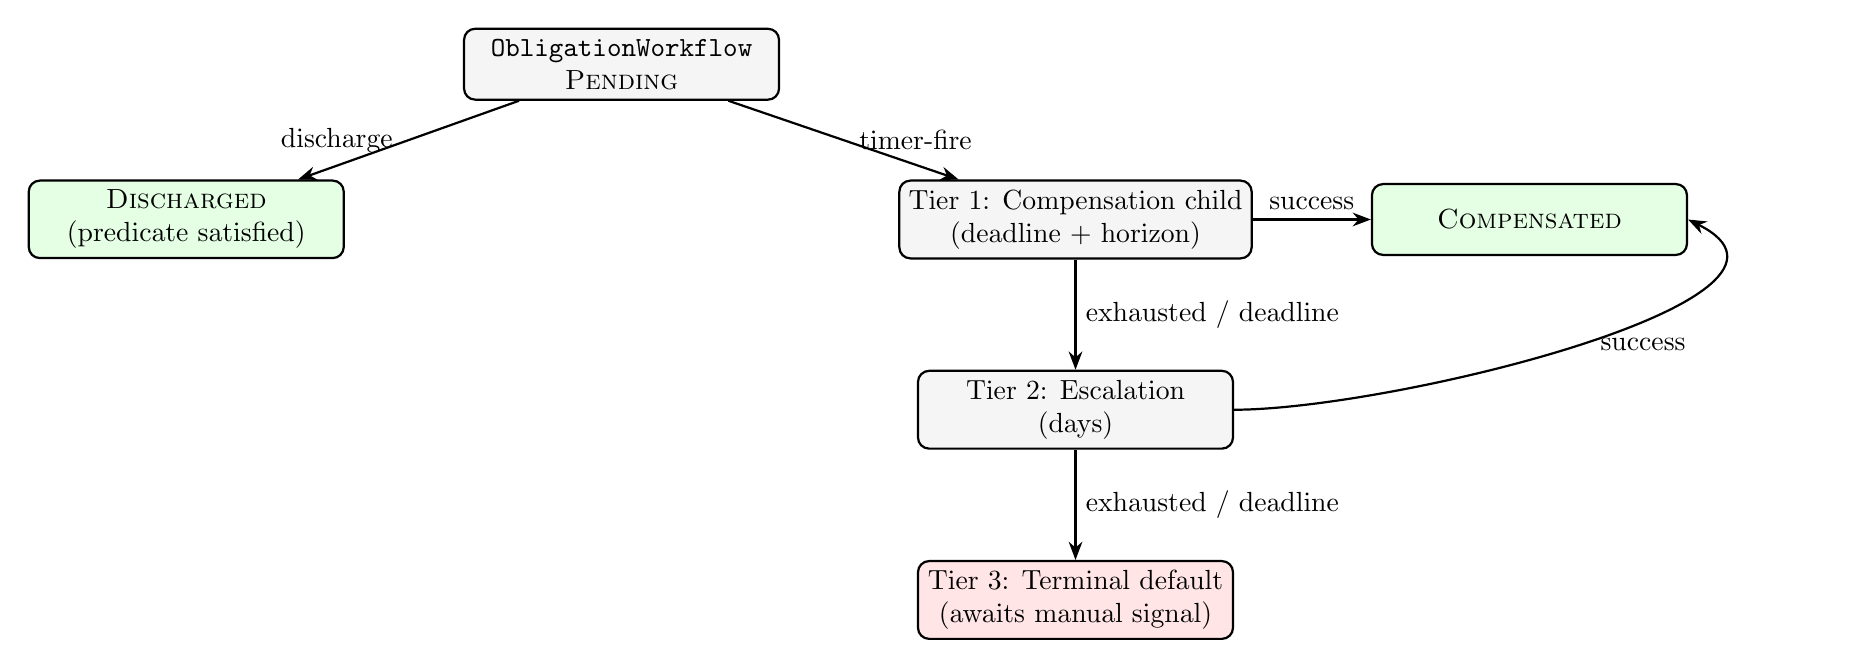
\begin{tikzpicture}[
  ->,>=Stealth,thick,
  every node/.style={align=center},
  block/.style={rectangle,draw,rounded corners,minimum width=4.0cm,minimum height=0.9cm,fill=gray!8},
  term/.style={rectangle,draw,rounded corners,minimum width=4.0cm,minimum height=0.9cm,fill=red!10},
  ok/.style={rectangle,draw,rounded corners,minimum width=4.0cm,minimum height=0.9cm,fill=green!10}
]
\node[block] (obl) {\texttt{ObligationWorkflow}\\\textsc{Pending}};
\node[ok,below left=1.0cm and 1.5cm of obl] (disc) {\textsc{Discharged}\\(predicate satisfied)};
\node[block,below right=1.0cm and 1.5cm of obl] (t1) {Tier 1: Compensation child\\(deadline + horizon)};
\node[block,below=1.4cm of t1] (t2) {Tier 2: Escalation\\(days)};
\node[term,below=1.4cm of t2] (t3) {Tier 3: Terminal default\\(awaits manual signal)};
\node[ok,right=1.5cm of t1] (cmp) {\textsc{Compensated}};
\draw (obl) -- node[left,xshift=-2pt]{discharge} (disc);
\draw (obl) -- node[right,xshift=2pt]{timer-fire} (t1);
\draw (t1) -- node[right]{exhausted / deadline} (t2);
\draw (t2) -- node[right]{exhausted / deadline} (t3);
\draw (t1) -- node[above]{success} (cmp);
\draw (t2.east) .. controls +(2,0) and +(2,-1) .. node[right,xshift=4pt]{success} (cmp.east);
\end{tikzpicture}
\end{center}

\paragraph{Late-discharge race policy.} The race --- a discharge signal arriving \emph{after} the deadline timer fired and compensation began --- is resolved per obligation kind. SBL recall, manufactured payment, locate confirmation, and buy-in confirmation: \emph{Reject} (deadline sacrosanct). Settlement and margin call: \emph{Cancel-compensation if compensation has not externalised; otherwise queue-and-reconcile}. Regulatory submission ack: \emph{Queue-and-reconcile}. Coupon / income event: \emph{Cancel-compensation}. The policy table is pinned per kind via the \emph{schema} axis of the VersionPinSidecar.

\subsection{Bitemporal Restatement Orchestration}
\label{sec:operational-restatement}

A single \texttt{RestatementWatchWorkflow} runs per $(\text{observable\_class}, \text{vendor})$ tuple, where the observable class lies in the closed sum
\[
\{\text{raw\_market}, \text{calibrated}, \text{fixing}, \text{corp\_action}, \text{calendar}, \text{party\_lei}, \text{ssi}, \text{tax\_form}\}.
\]
The workflow id format is \texttt{restate-watch:\{observable\_class\}:\{vendor\}}. Each instance subscribes to ``new-$t_{\mathrm{known}}$-for-prior-$t_{\mathrm{obs}}$'' events from the snapshot store, holds a paginated subscriber list in workflow state, fans out signals, tracks acknowledgements, retries unacked subscribers per a backoff policy, and continues-as-new at 8000 events or 30 days.

\paragraph{TikZ diagram of the workflow:}

\begin{center}
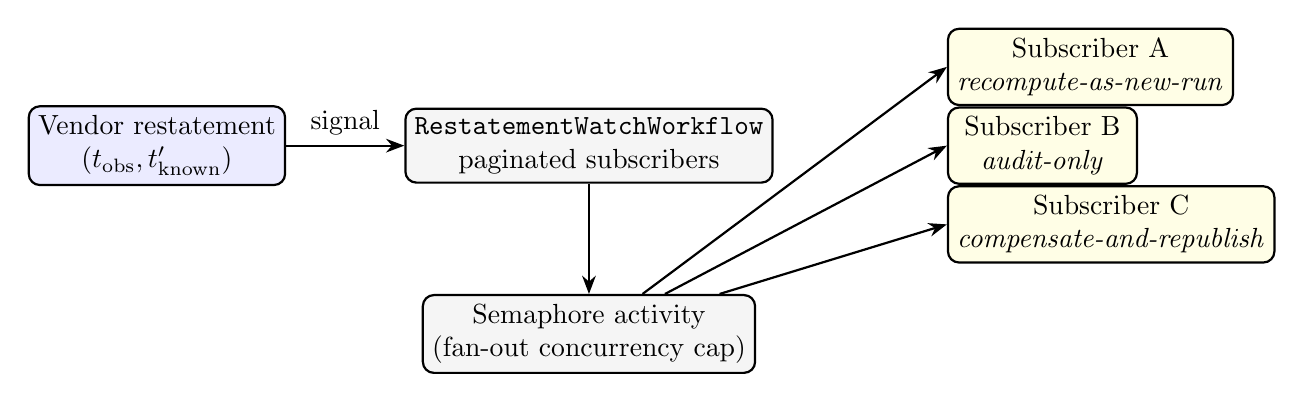
\begin{tikzpicture}[
  ->,>=Stealth,thick,
  every node/.style={align=center},
  src/.style={rectangle,draw,rounded corners,minimum width=2.6cm,minimum height=0.9cm,fill=blue!8},
  flow/.style={rectangle,draw,rounded corners,minimum width=3.6cm,minimum height=0.9cm,fill=gray!8},
  sub/.style={rectangle,draw,rounded corners,minimum width=2.4cm,minimum height=0.7cm,fill=yellow!10}
]
\node[src] (vendor) {Vendor restatement\\($t_{\mathrm{obs}}, t_{\mathrm{known}}'$)};
\node[flow,right=1.5cm of vendor] (rwf) {\texttt{RestatementWatchWorkflow}\\paginated subscribers};
\node[sub,right=2.2cm of rwf,yshift=1.0cm] (s1) {Subscriber A\\\emph{recompute-as-new-run}};
\node[sub,right=2.2cm of rwf] (s2) {Subscriber B\\\emph{audit-only}};
\node[sub,right=2.2cm of rwf,yshift=-1.0cm] (s3) {Subscriber C\\\emph{compensate-and-republish}};
\node[flow,below=1.4cm of rwf] (sem) {Semaphore activity\\(fan-out concurrency cap)};
\draw (vendor) -- node[above]{signal} (rwf);
\draw (rwf) -- (sem);
\draw (sem) -- (s1.west);
\draw (sem) -- (s2.west);
\draw (sem) -- (s3.west);
\end{tikzpicture}
\end{center}

A subscriber registers at the moment of consumption with a typed predicate \texttt{\{observable\_id, t\_obs\_range\}}. On each restatement matching the predicate, the subscriber takes one of three stances: \emph{audit-only}, \emph{recompute-as-new-run}, or \emph{compensate-and-republish}. The workflow does not decide; it routes. Calendar restatements use this same workflow under \texttt{observable\_class = calendar}; the mode-1 pin guarantees that already-fired timers are untouched.

\subsection{Retention Matrix}
\label{sec:operational-retention}

\begin{center}
\renewcommand{\arraystretch}{1.05}
\begin{longtable}{@{}p{1.0cm}p{0.7cm}p{0.9cm}p{1.0cm}p{1.4cm}p{1.0cm}p{1.0cm}p{1.0cm}p{1.6cm}p{2.4cm}@{}}
\toprule
\textbf{Leaf} & \textbf{SOX} & \textbf{MiFIR} & \textbf{EMIR} & \textbf{CFTC 49} & \textbf{BCBS} & \textbf{FRTB} & \textbf{CASS} & \textbf{DORA RTO/RPO} & \textbf{GDPR conflict rule} \\
\midrule
\endfirsthead
\toprule
\textbf{Leaf} & \textbf{SOX} & \textbf{MiFIR} & \textbf{EMIR} & \textbf{CFTC 49} & \textbf{BCBS} & \textbf{FRTB} & \textbf{CASS} & \textbf{DORA RTO/RPO} & \textbf{GDPR conflict rule} \\
\midrule
\endhead
\bottomrule
\endfoot
$L_1$ & 7y & 5y & 5y & life+5y & cycle & cap-hist & --- & 4h / 0   & LEI retained \\
$L_2$ & 7y & 5y & 5y & life+5y & ---   & ---      & --- & 4h / 1h  & --- \\
$L_3$ & 7y & 5y & 5y & life+5y & ---   & ---      & --- & 4h / 1h  & LEI retained; erasure deferred \\
$L_4$ & 7y & 5y & 5y & life+5y & ---   & cap-hist & --- & 24h / 24h& --- \\
$L_5$ & 7y & 5y & 5y & life+5y & cycle & cap-hist & 5y  & 1h / 0   & --- \\
$L_6$ & 7y & 5y & 5y & life+5y & cycle & cap-hist & 5y  & 1h / 0   & --- \\
$L_7^{\mathrm{P}}$ & 7y & 5y & 5y & life+5y & cycle & cap-hist & --- & 24h / 24h & --- \\
$L_8$ & 7y & 5y & 5y & life+5y & ---   & ---      & --- & 24h / 24h& Counterparty info retained \\
$L_9$ & 7y & 5y & 5y & life+5y & ---   & cap-hist & --- & 4h / 1h  & --- \\
$L_{10}$ & 7y & 5y & 5y & life+5y & cycle & ---   & --- & 1h / 0   & --- \\
$L_{11}$ & 7y & 5y & 5y & life+5y & cycle & ---   & --- & 1h / 0   & --- \\
$L_{12}$ & --- & 5y & --- & ---  & ---   & cap-hist & --- & 4h / 1h & --- \\
$L_{13}$ & 7y & 5y & 5y & life+5y & cycle & cap-hist & 5y & 0 / 0   & Pseudonymisation \\
$L_{14}$ & 7y & 5y & --- & ---   & cycle & cap-hist & --- & 1h / 0   & --- \\
$L_{15}$ & 7y & 5y & 5y & life+5y & cycle & ---    & 5y & 1h / 0   & --- \\
$L_{16}$ & 7y & 5y & 5y & life+5y & cycle & ---    & --- & 24h / 24h& --- \\
$L_{17}$ & --- & 5y & 5y & life+5y & ---  & cap-hist & --- & 4h / 1h & --- \\
$L_{18}$ & 7y & 5y & 5y & ---    & cycle & ---     & 5y & 24h / 24h & --- \\
$L_{19}$ & 7y & 5y & 5y & life+5y & ---  & ---      & --- & 0 / 0   & --- \\
\caption{Per-leaf retention horizons (SOX 7y; MiFIR 5y; EMIR 5y after expiry; CFTC Part 49 life of swap + 5y; BCBS 239 through-the-cycle; FRTB capital history; CASS / Rule 15c3-3 5y).}
\label{tab:retention}
\end{longtable}
\end{center}

\paragraph{Perpetual-issuance edge case.} For instruments with no maturity (perpetual bonds, evergreen mandates), the retention horizon is $\max(\text{applicable\_regulation\_horizon}, \text{position\_state\_non\_zero} + 7\mathrm{y})$.

\paragraph{GDPR-minimisation conflict resolution rule.} Regulatory retention preempts the GDPR right-to-erasure for fields covered by a retention obligation; non-mandatory personal data is minimised at issue.

\subsection{Service-Level Matrix}
\label{sec:operational-sla}

\begin{center}
\renewcommand{\arraystretch}{1.05}
\begin{longtable}{@{}p{1.0cm}p{1.6cm}p{1.6cm}p{6.0cm}p{1.4cm}p{1.4cm}@{}}
\toprule
\textbf{Leaf} & \textbf{p50} & \textbf{p99} & \textbf{Degraded mode} & \textbf{DORA RTO} & \textbf{DORA RPO} \\
\midrule
\endfirsthead
\toprule
\textbf{Leaf} & \textbf{p50} & \textbf{p99} & \textbf{Degraded mode} & \textbf{DORA RTO} & \textbf{DORA RPO} \\
\midrule
\endhead
\bottomrule
\endfoot
$L_1$    & 100 ms & 1 s    & Reject; manual review                                & 4 h  & 0    \\
$L_2$    & 1 s    & 10 s   & Stale-allowed marker; FSM \textsc{Stale} on dependents& 4 h  & 1 h  \\
$L_3$    & 1 s    & 10 s   & Stale-allowed for non-critical; reject new trades on lapsed LEI & 4 h  & 1 h  \\
$L_4$    & 1 s    & 10 s   & Reject pricing; FSM \textsc{Stale}                  & 24 h & 24 h \\
$L_5$    & 10 ms  & 100 ms & Reject reads; quorum-based                          & 1 h  & 0    \\
$L_6$    & 10 ms  & 100 ms & Reject reads; quorum-based                          & 1 h  & 0    \\
$L_7^{\mathrm{P}}$ & 100 ms & 1 s & Last-known-good with quality flag             & 24 h & 24 h \\
$L_8$    & 100 ms & 1 s    & Reject new trades; existing unaffected               & 24 h & 24 h \\
$L_9$    & 1 ms   & 10 ms  & FSM \textsc{Stale}; quality flag                     & 4 h  & 1 h  \\
$L_{10}$ & 100 ms & 1 s    & Defer to bilateral fallback; manual reconciliation   & 1 h  & 0    \\
$L_{11}$ & 100 ms & 1 s    & Stale-allowed; reconciliation queue                  & 1 h  & 0    \\
$L_{12}$ & 1 s    & 10 s   & FSM \textsc{Stale}; downgrade $L_{14}$ quality       & 4 h  & 1 h  \\
$L_{13}$ & 10 ms  & 100 ms & Reject commit; defer to manual review                & 0    & 0    \\
$L_{14}$ & 100 ms & 1 s    & FSM \textsc{Stale}                                   & 1 h  & 0    \\
$L_{15}$ & 100 ms & 1 s    & Saga compensation; escalation                        & 1 h  & 0    \\
$L_{16}$ & 1 s    & 10 s   & Stale-allowed                                        & 24 h & 24 h \\
$L_{17}$ & 1 s    & 10 s   & Queue; submit on recovery                            & 4 h  & 1 h  \\
$L_{18}$ & 100 ms & 1 s    & Aging proceeds; manual escalation                    & 24 h & 24 h \\
$L_{19}$ & 100 us & 1 ms   & Refuse pricing; FSM \textsc{Stale}                  & 0    & 0    \\
\caption{Per-leaf p50 / p99 ingress SLA, degraded mode, DORA RTO/RPO.}
\label{tab:sla}
\end{longtable}
\end{center}

\paragraph{T+1 affirmation.} $L_{11}$ affirmation must complete by 9pm ET on T+0. SLA p99 cutoff: 9pm ET on T+0 minus the settlement-orchestration buffer.

\paragraph{T+0 settlement (US equities post-2024).} $L_{11}$ confirmation must arrive by 11:30am ET on T (DTCC cutoff). Late confirmation triggers \texttt{wf-confirm-break} with a CSDR penalty obligation if cross-border.

\subsection{IPV / FRTB AVA on $L_{14}$}
\label{sec:operational-ipv}

The valuation record carries the IPV / FRTB AVA fields enumerated in Section~\ref{sec:leaf-l14}: \texttt{fair\_value\_level}, \texttt{ipv\_status}, \texttt{ipv\_variance}, \texttt{ipv\_source\_id}, \texttt{prudent\_valuation\_adjustment\_components} (with the seven sub-components: market-price uncertainty, close-out cost, model risk, concentrated position, future administrative costs, early termination, operational risk), \texttt{unobservable\_inputs[]}, \texttt{unobservable\_input\_sensitivity[]}.

\subsection{CSDR Penalty Schema}
\label{sec:operational-csdr}

The CSDR penalty kind is encoded as \texttt{obligation\_kind = CSDR\_PENALTY} with the schema $(\texttt{rate\_basis\_points}, \texttt{days}, \texttt{source\_lei}, \texttt{currency})$. The penalty fires on settlement-fail attestations from custodians or CCPs.

\subsection{Lineage Cursor}
\label{sec:operational-lineage}

The lineage cursor is a typed graph projection over $L_{13} \oplus L_{12} \oplus L_9 \oplus L_{10} \oplus \text{envelopes} \oplus \text{VersionPinSidecar} \oplus \text{capabilities}$ with materialised forward and reverse edges, supporting SOX \S404, BCBS 239 \S3, DORA Article 8, and IFRS 13 Level 3 query paths. Implemented as Datalog over content-addressed identities.

\clearpage
%==============================================================================
\section{Property-Based Testing Program}
\label{sec:pbt}
%==============================================================================

The data layer is verified by a stratified test pyramid in which every layer has a target count, a property kind, a generator strategy, and a coverage gate. Without a stratified pyramid the law $\Lambda_n$ becomes a paragraph rather than a property; without explicit coverage gates the test corpus drifts.

\subsection{Test Pyramid Declaration}
\label{sec:pbt-pyramid}

\begin{center}
\renewcommand{\arraystretch}{1.10}
\begin{tabular}{@{}p{3.0cm}p{2.5cm}p{2.5cm}p{3.5cm}p{3.5cm}@{}}
\toprule
\textbf{Layer} & \textbf{Target count} & \textbf{Property kind} & \textbf{Generator strategy} & \textbf{Coverage gate} \\
\midrule
Unit ($\Phi_n$ per leaf)  & $\sim 640$ (16 families $\times \sim 40$) & Type-level     & Hypothesis / proptest over closed sums & 100\% (mandatory) \\
Property (per $\Lambda_n$)& 15                                       & Cross-layer    & Stratified per coverage targets       & Per-stratum assertions \\
Mutation                  & $\sim 750$ ($15 \text{ ops} \times 50$ sites) & Mutation testing & \texttt{mutmut} / \texttt{cosmic-ray} & Stratified kill-rate \\
Saga / chaos              & $\sim 30$                                 & End-to-end     & \texttt{temporal-test-server} + Buggify & Determinism replay \\
Boundary ($B_1$--$B_{17}$)& 17                                       & I/O integration& Recorded fixtures                      & Per-boundary CI test \\
Regression fixture corpus & $\ge 40$                                  & Characterisation & Recorded-replay                      & 100\% retained as guards \\
\bottomrule
\end{tabular}
\end{center}

The CI gate fails on any layer below its target count.

\subsection{Property Oracle for $\Lambda_1$}
\label{sec:pbt-oracle}

The genuinely-unwitnessed status of $\Lambda_1$ stands on the impossibility of provably establishing vendor honesty under composition. The runtime obligation is decidable, however, via the trust-registry surrogate:

\begin{lstlisting}
property P-Lambda1-VENDOR-OPACITY (tx: Transaction):
  for each input observation o in tx.lineage:
    assert TrustRegistry.contains(o.attestor)
    assert TrustRegistry[o.attestor].status == ACTIVE
    if o.aggregation_outcome == single_source_authority:
      assert o.single_source_authority_assumption_ref
              in TrustRegistry
      assert TrustRegistry.last_review[o.attestor]
              within review_cadence
    else:
      assert o.aggregation_outcome
              in {multi_source_consensus, quarantined}
\end{lstlisting}

The property runs at every commit boundary, in $\mathcal{O}(|\text{tx.lineage}| \cdot \log |\text{TrustRegistry}|)$. False under: unregistered attestor, killed attestor, lapsed review, single-source admission without registered exception. Kill-switch: a registry status flip from \textsc{Active} to \textsc{Killed} quarantines all post-attestor data and triggers replay re-verify against alternate sources.

\subsection{HWM-Cross-Mandate-Collapse Fixture}
\label{sec:pbt-hwm}

\begin{lstlisting}
fixture HWM-COLLAPSE-1 (Lambda_6 violation candidate):
  setup:
    mandate_A = create_mandate(qis=A, hwm=100, fee_pct=0.20)
    mandate_B = create_mandate(qis=B, hwm=100, fee_pct=0.20)
    move(client_C -> mandate_A, units=10)
    move(client_C -> mandate_B, units=10)
  trigger:
    nav_update(mandate_A, new_nav=120)
    nav_update(mandate_B, new_nav=80)
    crystallise_fee(mandate_A)
    nav_update(mandate_A, new_nav=80)
  assertion:
    assert hwm[mandate_A] != hwm[mandate_B]
    assert fee_accrual[mandate_A] >= 4
    assert fee_accrual[mandate_B] == 0
\end{lstlisting}

Plus four variant fixtures: cross-currency QIS; manufactured-payment cross-jurisdiction; tax-treatment-divergent QIS; mandate-as-unit-being-superseded mid-crystallisation.

\subsection{Mutation Kill-Rate Floors}
\label{sec:pbt-mutation}

Stratified kill-rate floors by ($\Lambda$-cluster $\times$ mutation operator). Bold cells are critical: survivors fail the build. Other cells are advisory floors; survivors generate review-required findings.

\begin{center}
\scriptsize
\renewcommand{\arraystretch}{1.05}
\begin{longtable}{@{}p{3.2cm}*{15}{p{0.55cm}}@{}}
\toprule
\textbf{Cluster} & \textbf{CONS} & \textbf{BND} & \textbf{VAC} & \textbf{CLK} & \textbf{CCH} & \textbf{NPJ} & \textbf{CAN} & \textbf{CDM} & \textbf{CAP} & \textbf{LAT} & \textbf{FCT} & \textbf{AGG} & \textbf{DFL} & \textbf{BIA} & \textbf{SHR} \\
\midrule
\endfirsthead
\toprule
\textbf{Cluster} & \textbf{CONS} & \textbf{BND} & \textbf{VAC} & \textbf{CLK} & \textbf{CCH} & \textbf{NPJ} & \textbf{CAN} & \textbf{CDM} & \textbf{CAP} & \textbf{LAT} & \textbf{FCT} & \textbf{AGG} & \textbf{DFL} & \textbf{BIA} & \textbf{SHR} \\
\midrule
\endhead
\bottomrule
\endfoot
$\Lambda_5/\Lambda_6/\Lambda_7/\Lambda_{15}$ & \textbf{95} & 80 & 90 & 50 & 90 & 95 & 80 & 80 & 80 & 50 & 80 & \textbf{95} & 90 & 70 & 60 \\
$\Lambda_1/\Lambda_2/\Lambda_8$              & 80 & 80 & 80 & 80 & \textbf{95} & 80 & 80 & 80 & 80 & 70 & 80 & 80 & 80 & 70 & 70 \\
$\Lambda_{11}/\Lambda_{12}$                  & 80 & 80 & 80 & 70 & 80 & 80 & 80 & 80 & 70 & 70 & \textbf{95} & 80 & \textbf{95} & \textbf{90} & 70 \\
$\Lambda_{13}$                                & 80 & 80 & 80 & 80 & 80 & 80 & 80 & 80 & 80 & \textbf{95} & 80 & 80 & 80 & 70 & \textbf{90} \\
$\Lambda_4$                                   & 80 & 80 & 80 & 80 & \textbf{95} & 80 & 80 & 80 & 80 & 80 & 80 & 80 & 80 & 70 & 70 \\
$\Lambda_{14}$                                & 80 & 80 & 80 & 80 & 80 & 80 & 80 & 80 & \textbf{95} & 80 & 80 & 80 & 80 & 70 & 70 \\
\caption{Mutation kill-rate floors (\%) by ($\Lambda$-cluster $\times$ operator). Bold cells are critical.}
\label{tab:mutation-floors}
\end{longtable}
\end{center}

\clearpage
%==============================================================================
\section{Goodhart Hardening}
\label{sec:goodhart}
%==============================================================================

A specification is a target; a target invites optimisation; optimisation against a target without honesty is Goodhart's law in action. The data layer hardens against five named traps. Each trap is paired with a detection mechanism.

\begin{center}
\renewcommand{\arraystretch}{1.15}
\begin{tabular}{@{}p{0.8cm}p{4.5cm}p{9.5cm}@{}}
\toprule
\textbf{\#} & \textbf{Trap} & \textbf{Detection / avoidance mechanism} \\
\midrule
$\mathrm{GT}_1$ & Snapshot stub-swap & Boundary-integrity production test: pull $N$ committed transactions from the production snapshot store; replay; assert byte-identical \\
$\mathrm{GT}_2$ & Mutation-set exclusion & Fifteen mutation operators with mandatory survivor reporting and stratified kill-rate targets (Section~\ref{sec:pbt-mutation}) \\
$\mathrm{GT}_3$ & Biased generators & First-class coverage targets per stratum: 5\% near-arbitrage-boundary, 10\% deadline-near-fire, 10\% multi-CCP, 5\% manufactured-payment-cross-jurisdiction. CI-asserted. \\
$\mathrm{GT}_4$ & Aggregation-masking & Meta-property: aggregation tests must pass at every per-class projection, not only globally \\
$\mathrm{GT}_5$ & Type-system witness laundering & Three-layer defence: (a) type system with strict checker plus AST lint banning \texttt{cast} / \texttt{\_\_new\_\_} outside the constructor module; (b) runtime checker on every write attempt; (c) adversarial Hypothesis test attempting reflection / \texttt{\_\_post\_init\_\_} bypass. Closed witness inventory $W_1$--$W_5$ enumerates construction, consumer, and elimination sites \\
\bottomrule
\end{tabular}
\end{center}

The witness inventory $W_1$ \texttt{arbitrage\_certificate}; $W_2$ \texttt{snapshot\_certificate}; $W_3$ \texttt{conserving\_transaction} / \texttt{balanced\_transaction}; $W_4$ \texttt{registered\_unit\_id}; $W_5$ \texttt{calibrated\_state} (GADT-keyed by model). Each witness has a single construction site and is consumed by exhaustive pattern match.

\clearpage
%==============================================================================
\section{Surfaced Disagreements: Plain Rulings}
\label{sec:disagreements}
%==============================================================================

The five structural disagreements surfaced during the construction of this document are recorded as plain rulings. The ``tension box'' format (presenting two positions in parallel without a decision) is forbidden.

\begin{description}[style=nextline]
\item[$D_1$ Leaf count] Resolution: nineteen leaves (Sections~\ref{sec:taxonomy}). ADR-2, ADR-3, ADR-4. No alternative tolerated.
\item[$D_2$ Tokenised collateral framing] Resolution: \texttt{lifecycle\_model = SmartContract} on $L_1$ plus \texttt{EligibleCollateralCriteria} extension in CDM. \texttt{DigitalAsset} excluded by live CDM. ADR-10. No alternative tolerated.
\item[$D_3$ Surrogate witnesses] Resolution: $\Lambda_1$ is genuinely unwitnessed under vendor opacity, accepted as architectural risk with named owners (CRO + Head of Reference Data); the runtime obligation is discharged by the property oracle of Section~\ref{sec:pbt-oracle}. $\Lambda_4, \Lambda_8, \Lambda_{13}$ are witnessed via composition with bounded parameters specified in the realism budget.
\item[$D_4$ Stored caches $L_5$, $L_6$] Resolution: ADR-1 carve-out of veto $V_{13}$ citing StatesHome $C_{11}$. Cache-invalidation discipline $\mathrm{CIv}\textrm{-}1, \mathrm{CIv}\textrm{-}2, \mathrm{CIv}\textrm{-}3$ per Theorem~\ref{thm:cache-coh}. No alternative tolerated.
\item[$D_5$ Compensations] Resolution: three-tier saga tower (compensation child workflow $\to$ escalation workflow $\to$ terminal default). Trivial compensations remain activities. ADR-8.
\end{description}

\clearpage
%==============================================================================
\section{Architecture Decision Register}
\label{sec:adr}
%==============================================================================

\begin{center}
\renewcommand{\arraystretch}{1.10}
\begin{longtable}{@{}p{1.0cm}p{4.6cm}p{2.8cm}p{6.5cm}@{}}
\toprule
\textbf{ADR} & \textbf{Title} & \textbf{Veto / Leaf} & \textbf{Justification} \\
\midrule
\endfirsthead
\toprule
\textbf{ADR} & \textbf{Title} & \textbf{Veto / Leaf} & \textbf{Justification} \\
\midrule
\endhead
\bottomrule
\endfoot
ADR-1  & $L_5/L_6$ stored cache override of $V_{13}$ & $V_{13}$ & StatesHome $C_{11}$ single-writer invariant; cache-invalidation discipline $\mathrm{CIv}\textrm{-}1/2/3$ per Th-4b \\
ADR-2  & $L_{17}$ RegulatorySubmission elevation & New leaf & CFTC, EMIR Refit, SFTR, SLATE, MiFIR RTS 22, FRTB Pillar 3; DRR rule-set version pin \\
ADR-3  & $L_{18}$ BreakRegister elevation & New leaf & SOX \S404; BCBS 239 \S3; DORA Article 8 \\
ADR-4  & $L_{19}$ ClockAuthority elevation & New leaf & Time-translation invariance carrier; replay determinism \\
ADR-5  & Mode-1 calendar amendment pin & $L_4$ & Preserves time-translation invariance; calendar republication produces new bitemporal record but does not invalidate prior pins \\
ADR-6  & Canonicalisation pin (RFC 8785 JCS / Protobuf canonical / CBOR per RFC 8949) & VersionPinSidecar / $B_{10}$ & Cross-implementation replay determinism \\
ADR-7  & \texttt{tx\_id} formula excludes \texttt{run\_id} & $L_{13}$ & $\texttt{ContinueAsNew}$ changes \texttt{run\_id}; old formula breaks idempotency \\
ADR-8  & Compensation workflows for non-trivial obligations & $L_{15}$ & Three-tier saga tower; trivial compensations remain activities \\
ADR-9  & Single-source admission via $N_{8.2}$ explicit assumption ref & $L_9$ & Vendor honesty $\mathrm{C\textrm{-}A}_3$ named assumption; multi-source default \\
ADR-10 & Tokenised collateral via \texttt{lifecycle\_model = SmartContract} on $L_1$ + \texttt{EligibleCollateralCriteria} extension & $L_1$ / CDM & \texttt{DigitalAsset} rejected by live CDM (\texttt{assetType = Other} excludes tokenised) \\
ADR-11 & Public verification keys append-only & $B_{11}$ & HSM rotation discipline; replay re-verify of old envelopes \\
ADR-12 & $L_7^{\mathrm{Pa/b/c}}$ partition with $\le 30$ fields per partition & $L_7^{\mathrm{P}}$ & Veto $V_9$ enforcement via CI \\
\caption{Architecture decision register.}
\label{tab:adr}
\end{longtable}
\end{center}

\clearpage
%==============================================================================
\section{Lines-of-Code Budget}
\label{sec:loc}
%==============================================================================

A specification that does not bind itself to an implementation budget invites over-engineering. The budget below is normative; an implementation that exceeds the hard cap signals a defect in the specification, not (only) in the implementation.

\begin{center}
\renewcommand{\arraystretch}{1.15}
\begin{tabular}{@{}p{8cm}p{3.5cm}p{3.5cm}@{}}
\toprule
\textbf{Component} & \textbf{Budget} & \textbf{Hard cap} \\
\midrule
Core Ledger types (closed sums + smart constructors + parsers) & 3{,}000 LoC & 5{,}000 LoC \\
Core Ledger handlers (per (event\_class $\times$ obligation\_kind) cell) & 2{,}500 LoC & 4{,}000 LoC \\
Core executor + chain logic & 1{,}500 LoC & 2{,}500 LoC \\
\textbf{Total core implementation} & \textbf{$\le$ 7{,}000 LoC} & \textbf{$\le$ 10{,}000 LoC} \\
Vendor adapters (one per vendor / source; $\sim 10$ sources) & $\sim 500$ LoC each & $\sim 6{,}000$ LoC \\
Test suite (unit + property + saga + regression) & $\sim 12{,}000$ LoC & $\sim 20{,}000$ LoC \\
\textbf{Total system (core + adapters + tests)} & \textbf{$\le$ 25{,}000 LoC} & \textbf{$\le$ 30{,}000 LoC} \\
\bottomrule
\end{tabular}
\end{center}

\paragraph{Refactoring discipline.} Every new abstraction must justify itself against the cap. If the implementation overflows the hard cap, the specification is wrong: review for premature abstraction, leaf-count creep, or a missing closed-sum.

\clearpage
%==============================================================================
\section{Verification Approach}
\label{sec:verification}
%==============================================================================

The data layer is verified by ten audit steps. The first six are mechanical (CI-enforced); the last four are governance steps performed at quarterly cadence at minimum.

\begin{enumerate}[nosep,leftmargin=*]
\item \textbf{Per-veto CI mechanism inventory.} For each $V_n$, verify the falsifying-predicate test exists, runs on every commit, and has been observed to fail at least once during development.
\item \textbf{Per-boundary CI test.} For each $B_n$, verify the boundary integration test runs on every commit and the recorded fixture is byte-identical to the production snapshot.
\item \textbf{Theorem hypothesis totality.} For each $\mathrm{Th}\textrm{-}n$, verify every quantifier range is explicit and every base case is stated; the dependency DAG is acyclic.
\item \textbf{Surrogate parameters specified.} For each witnessed-via-composition law, verify the parameter is recorded in $L_7^{\mathrm{Pb}}$ and observable in production: $\Lambda_4$ retention horizon $\kappa_{\mathrm{restate}}$; $\Lambda_8$ erasure-coding $(n,k,\varepsilon)$; $\Lambda_{13}$ $T_{\max}$ and $\delta_{\mathrm{h}}$.
\item \textbf{CDM cross-walk re-fetch.} The Direct / Partial / Missing labels reflect live FINOS CDM 6.0.0; suspect path/type claims have been resolved against the canonical source.
\item \textbf{Versioning Algebra composition rules.} For each $\Lambda_n$, the required pin axes are stated; mutation tests verify that flipping a pin breaks the law.
\item \textbf{Operational floor matrices are normative.} Reconciliation, retention, SLA, IPV: each row is owned by a named team; each cell has been reconciled against an external authoritative source.
\item \textbf{Trust-assumption registry artefact.} The thirteen conditional assumptions are rows in the registry; the schema, review cadence, and kill-switch are real (not paragraphs).
\item \textbf{Mutation kill-rate stratified report.} Bold cells of Section~\ref{sec:pbt-mutation} are CI-blocking; advisory cells are reviewed quarterly.
\item \textbf{Goodhart trap detection.} Each of $\mathrm{GT}_1, \dots, \mathrm{GT}_5$ has at least one production-attempted test that has failed during development and been remediated; the witness inventory $W_1$--$W_5$ is current.
\end{enumerate}

\clearpage
%==============================================================================
\section{Glossary}
\label{app:glossary}
%==============================================================================

The following terms are used throughout this document with specific technical meanings.

\begin{description}[style=nextline]
\item[Attestor] An external authority (vendor, regulator, calculation agent, custodian, CCP) whose statements enter the Ledger only through a bitemporal observation leaf with a verified signature.
\item[BCBS 239] Basel Committee paper on risk data aggregation and reporting; cited for the through-the-cycle retention requirement and break-management discipline.
\item[Bitemporal axes] The pair $(t_{\mathrm{obs}}, t_{\mathrm{known}})$ on every record in $C_1 \cup C_4$; mandatory two-axis indexing.
\item[BreakRegister] Leaf $L_{18}$; mutable break record with the FSM of Section~\ref{sec:operational-fsm}.
\item[CDM] FINOS Common Domain Model, expressed in the Rosetta DSL.
\item[ContinueAsNew] Temporal SDK construct that closes a workflow run and starts a new run with a transformed payload, preserving idempotency keys.
\item[Conservation] The ledger invariant $\sum_w w(u) = 0$ per unit class; the structural sum is enforced by handler type-tagging.
\item[CRR Article 105 PVA] EU Capital Requirements Regulation Article 105 prudent valuation adjustments; reflected in $L_{14}$ \texttt{prudent\_valuation\_adjustment\_components}.
\item[CSDR] EU Central Securities Depositories Regulation; settlement-fail penalty regime on cross-border settlement.
\item[DORA] EU Digital Operational Resilience Act; Article 8 break-management; RTO/RPO matrix in Section~\ref{sec:operational-sla}.
\item[DRR] Digital Regulatory Reporting (CDM-native rule sets); pinned per the versioning algebra axis \texttt{drr\_rule\_set\_pin}.
\item[EMIR Refit] EU European Market Infrastructure Regulation refit; transaction reporting.
\item[FpML] Financial products Markup Language; XML schema for OTC derivatives; an inbound wire format for $L_{11}$.
\item[FRTB AVA] Fundamental Review of the Trading Book Additional Valuation Adjustments; the seven AVA categories on $L_{14}$.
\item[FRTB PLA] Fundamental Review of the Trading Book PnL Attribution test.
\item[IPV] Independent Price Verification.
\item[ISDA Notices Hub] Industry hub for ISDA Master Agreement default and termination notices.
\item[JCS canonicalisation] JSON canonicalisation per RFC 8785; pinned at boundary $B_{10}$.
\item[KIKO] Knock-In / Knock-Out; an option lifecycle pattern.
\item[$\Lambda$-laws] The fifteen cross-cutting consistency laws of Section~\ref{sec:laws}.
\item[Mandate-as-unit] Modelling pattern in which a mandate (e.g.\ a managed account or QIS strategy) is itself a unit in $\mathcal{U}$; cf.~\cite[StatesHome]{ledger}.
\item[MiFIR] EU Markets in Financial Instruments Regulation; transaction reporting under RTS 22.
\item[MoveStream] Leaf $L_{13}$; canonical hash-chained sequence of \texttt{BalancedTransaction}.
\item[Pricing DAG] Directed acyclic graph of pricing dependencies (cf.~\cite[\S6]{valuation}).
\item[ProductTerms] Leaf $L_1$; StatesHome map 1.
\item[QIS] Quantitative Investment Strategy unit type.
\item[RestatementWatchWorkflow] The bitemporal-restatement orchestration of Section~\ref{sec:operational-restatement}.
\item[SFTR] EU Securities Financing Transactions Regulation.
\item[SLATE] FINRA Securities Lending and Transparency Engine.
\item[SOX] US Sarbanes-Oxley Act \S404; control discipline for financial reporting.
\item[StatesHome 3-map] The three maps \texttt{ProductTerms} ($L_1$), \texttt{UnitStatus} ($L_5$), $\texttt{PositionState}[(w,u)]$ ($L_6$).
\item[$\Theta_{\mathrm{AF}}$] Model-versioned no-arbitrage admissible parameter set; $\Theta_{\mathrm{AF}}: (\text{model\_id} \times \text{model\_version}) \to \text{AdmissibleSet}$.
\item[UnitStatus] Leaf $L_5$; StatesHome map 2.
\item[$\Phi$-invariants] Per-leaf invariant families with type ($T$), workflow ($W$), and composition ($C$) variants.
\end{description}

\vspace{2em}
\noindent\rule{\textwidth}{0.4pt}

\noindent\textbf{Document Version:} v1.0\\
\textbf{Date:} April 2026\\
\textbf{Classification:} Design Specification

\clearpage
%==============================================================================
\begin{thebibliography}{9}

\bibitem{ledger}
R.~Delloye, ``The Ledger: A Closed-System Framework for Financial Settlement --- Unified Design Specification: Architecture, Lifecycle, and CDM Integration,'' v10.3, March~2026.

\bibitem{valuation}
R.~Delloye, ``The Ledger Valuation Stack: Pricing, Greeks, Calibration, PnL Attribution, and Temporal Orchestration,'' v1.0, March~2026.

\end{thebibliography}

\end{document}
